\documentclass[11pt,a4paper]{tesis}

\usepackage{thesis}
\usepackage{sections/nd_rules}

% Para solo agregar algunas secciones
% \includeonly{
%     sections/intro,
%     sections/natural_deduction,
%     sections/ppa,
%     sections/ppa_certifier
% }

\begin{document}
%%%% CARATULA

\def\autor{Manuel Panichelli}
\def\tituloTesis{
PPA - Un asistente de demostración para lógica de primer orden con extracción de
testigos usando la traducción de Friedman
}
\def\runtitulo{PPA - Un asistente de demostración para lógica de primer orden
con extracción de testigos usando la traducción de Friedman}
\def\runtitle{PPA - a proof-assistant for first-order logic with witness extraction using Friedman's translation}
\def\director{Pablo Barenbaum}
\def\lugar{Buenos Aires, 2024}

\newcommand{\HRule}{\rule{\linewidth}{0.2mm}}
%
\thispagestyle{empty}

\begin{center}\leavevmode

\vspace{-2cm}

\begin{tabular}{l}

\includegraphics[width=2.6cm]{logofcen.pdf}
\end{tabular}


{\large \sc Universidad de Buenos Aires

Facultad de Ciencias Exactas y Naturales

Departamento de Computaci\'on}

\vspace{6.0cm}

%\vspace{3.0cm}
%{
%\Large \color{red}
%\begin{tabular}{|p{2cm}cp{2cm}|}
%\hline
%& Pre-Final Version: \today &\\
%\hline
%\end{tabular}
%}
%\vspace{2.5cm}

\begin{huge}
\textbf{\tituloTesis}
\end{huge}

\vspace{2cm}

{\large Tesis de Licenciatura en Ciencias de la Computaci\'on}

\vspace{2cm}

{\Large \autor}

\end{center}

\vfill

{\large

{Director: \director}

\vspace{.2cm}

{Codirector: \codirector}

\vspace{.2cm}

\lugar
}

\newpage\thispagestyle{empty}


\frontmatter
\pagestyle{empty}
%\begin{center}
%\large \bf \runtitulo
%\end{center}
%\vspace{1cm}
\chapter*{\runtitulo}

\noindent Los \textit{asistentes de demostración} son programas que simplifican
la escritura de demostraciones matemáticas, permitiendo la colaboración masiva o
la verificación formal de programas. Existen muchos asistentes como Mizar, Coq e
Isabelle, basados en distintas teorías. Un criterio deseable que pueden cumplir
es el de De Bruijn: a partir de demostraciones en un lenguaje de alto nivel se pueden extraer demostraciones en un lenguaje núcleo fácilmente verificable. Esto elimina la necesidad de tener que confiar en la implementación del asistente, ya que las demostraciones pueden ser verificadas por un programa independiente.

En esta tesis se presenta PPA, un asistente de demostración para lógica clásica
de primer orden. Cumple con el criterio de De Bruijn, generando demostraciones
en el sistema lógico de \textit{deducción natural} a partir de programas
escritos en un lenguaje de alto nivel, cuyo objetivo es ser similar a cómo
serían en lenguaje natural. Tiene un mecanismo principal de demostración, el \texttt{by},
que por debajo cuenta con un \textit{solver} heurístico para lógica de primer
orden que facilita la escritura de demostraciones. Está inspirado en el
mecanismo análogo en Mizar.

Algunos asistentes implementan la \textit{extracción de testigos de
existencial}. Dada una demostración de $\exists \var . \pred(\var)$, se extrae
un \textit{testigo} $\term$ tal que cumpla $\pred(\term)$. Es sencillo hacerlo sobre lógica intuicionista por su naturaleza constructiva, pero un desafío sobre lógica clásica, que no lo es. Para ello hay dos grandes categorías: directas (mediante técnicas semánticas como realizabilidad clásica \cite{miquel-friedman}) o indirectas (mediante traducciones a otra lógica, como intuicionista).

El aporte principal del trabajo es una implementación práctica de la extracción
de testigos. PPA la implementa de forma indirecta usando la traducción de
Friedman, que permite convertir  demostraciones clásicas de fórmulas
$\classPiTwo$ de la forma $\forall \varTwo_0 \dots \forall \varTwo_n . \exists
\var . \anyForm$ a demostraciones intuicionistas. Se describe cómo una vez traducidas pueden
ser normalizadas usando reglas de reducción bien conocidas, que se corresponden con las reglas de reducción del cálculo lambda vistas desde el isomorfismo
Curry-Howard. Finalmente, de una demostración normalizada se podrá extraer un
testigo. Identificamos algunos detalles en la implementación práctica de la
traducción, que limitan las fórmulas para las cuales se puede usar (más allá de
la limitación teórica de $\classPiTwo$) y también limitan las axiomatizaciones
de las teorías que se pueden hacer.

\bigskip

\noindent\textbf{Palabras claves:} asistente de demostración, lógica de primer orden, deducción natural, lógica clásica, lógica intuicionista, extracción de testigos, traducción de Friedman.

\cleardoublepage
%\begin{center}
%\large \bf \runtitle
%\end{center}
%\vspace{1cm}
\chapter*{\runtitle}

\noindent \textit{Proof assistants} are programs that simplify the writing of
mathematical proofs, enabling large-scale collaboration or the formal
verification of programs. There are many proof assistants such as Mizar, Coq,
and Isabelle, based on different theories. A desirable property they may have is
described by the De Bruijn criterion: from proofs written in a high level
language, one can extract proofs in a core, easily verifiable language. This
eliminates the need to trust their implementation, as the extracted proofs can
be verified by an independent program.

This thesis presents \textit{PPA}, a proof assistant for classical first-order logic. It fulfills De Bruijn's criterion by generating proofs in the natural deduction proof system from high-level proofs, designed to resemble natural language as closely as possible. Its main proof mechanism, \texttt{by}, features an underlying heuristic solver for first-order logic, inspired by Mizar's analogous mechanism.

Some proof assistants implement \textit{existential witness extraction}. Given a
proof of $\exists \var . \pred(\var)$, they extract a *witness* \( \term \) such
that \( \pred(\var) \) holds. While this is straightforward in intuitionistic
logic due to its constructive nature, it is challenging in classical logic,
which lacks constructiveness. There are two main approaches: direct (using
semantic techniques such as classical realizability \cite{miquel-friedman}) or indirect
(via translations to another logic, such as intuitionistic).

The main contribution of this work is a practical implementation of witness
extraction. PPA achieves this indirectly by using Friedman's translation, which
allows converting classical proofs of \( \classPiTwo \) formulas of the form \(
\forall y_0 \dots \forall y_n . \exists x . \anyForm \), with the formula
$\anyForm$ having no quantifiers, into intuitionistic ones. We
describes how, once translated, these proofs can be normalized using well-known
reduction rules, which correspond to the reduction rules of lambda calculus viewed through the Curry-Howard isomorphism. Finally, a
normalized proof enables the extraction of a witness. We identify some practical
implementation details of the translation, which limit the formulas for which it
can be used (beyond the theoretical \( \classPiTwo \) restriction) and also
constrain the axiomatizations of theories that can be made.

\bigskip

\noindent\textbf{Keywords:} proof assistant, first-order logic, natural deduction, classical logic, intuitionistic logic, witness extraction, Friedman's translation.

\cleardoublepage
\chapter*{Agradecimientos}

\noindent Lorem ipsum dolor sit amet, consectetur adipiscing elit. Fusce sapien ipsum, aliquet eget convallis at, adipiscing non odio. Donec porttitor tincidunt cursus. In tellus dui, varius sed scelerisque faucibus, sagittis non magna. Vestibulum ante ipsum primis in faucibus orci luctus et ultrices posuere cubilia Curae; Mauris et luctus justo. Class aptent taciti sociosqu ad litora torquent per conubia nostra, per inceptos himenaeos. Mauris sit amet purus massa, sed sodales justo. Mauris id mi sed orci porttitor dictum. Donec vitae mi non leo consectetur tempus vel et sapien. Curabitur enim quam, sollicitudin id iaculis id, congue euismod diam. Sed in eros nec urna lacinia porttitor ut vitae nulla. Ut mattis, erat et laoreet feugiat, lacus urna hendrerit nisi, at tincidunt dui justo at felis. Class aptent taciti sociosqu ad litora torquent per conubia nostra, per inceptos himenaeos. Ut iaculis euismod magna et consequat. Mauris eu augue in ipsum elementum dictum. Sed accumsan, velit vel vehicula dignissim, nibh tellus consequat metus, vel fringilla neque dolor in dolor. Aliquam ac justo ut lectus iaculis pharetra vitae sed turpis. Aliquam pulvinar lorem vel ipsum auctor et hendrerit nisl molestie. Donec id felis nec ante placerat vehicula. Sed lacus risus, aliquet vel facilisis eu, placerat vitae augue.


\cleardoublepage
\tableofcontents

\mainmatter
\pagestyle{headings}

%%%% CONTENIDO DE LA TESIS

\chapter{Introducción}



En este trabajo implementamos una asistente de demostración ``PPA''
(\textit{Pani's proof assistant}) inspirado en Mizar.

PPA se puede referir a varias cosas: el lenguaje para escribir demostraciones,
la herramienta (junto con su extracción de testigos).


\section{Teoremas}

In mathematics and formal logic, a theorem is a statement that has been proven, or can be proven.[a][2][3] The proof of a theorem is a logical argument that uses the inference rules of a deductive system to establish that the theorem is a logical consequence of the axioms and previously proved theorems.

In mainstream mathematics, the axioms and the inference rules are commonly left implicit, and, in this case, they are almost always those of Zermelo–Fraenkel set theory with the axiom of choice (ZFC), or of a less powerful theory, such as Peano arithmetic.[b] Generally, an assertion that is explicitly called a theorem is a proved result that is not an immediate consequence of other known theorems. Moreover, many authors qualify as theorems only the most important results, and use the terms lemma, proposition and corollary for less important theorems.

Completar con https://en.wikipedia.org/wiki/Theorem

\section{Asistentes de demostraciones}

\begin{itemize}
    \item Son programs que asisten al usuario a la hora de escribir una
    demostración. Permiten representarlas en un programa.
    \item Aplicaciones: formalización de teoremas, verificación formal de
    programas, etc.
    \item Ejemplos: Coq, isabelle (isar), Mizar
    \item Reseña histórica de Mizar
    \item Ventajas: colaboración a gran escala (confianza en el checker),
    chequear el output de los LLMs
\end{itemize}

\section{Arquitectura de PPA}

\begin{itemize}
    \item Por qué certificados (criterio de De Brujin)
    \item Certificados están en deducción natural. Sistema lógico que permite
    construir demostraciones mediante reglas de inferencia.
    \item PPA es un lenguaje que genera demostraciones "de bajo nivel" ND.
    \item razón de ser: Más práctico que demos de bajo nivel
    \item Implementado en Haskell
\end{itemize}

Principalmente hace dos cosas: certificar y extraer testigos.

\section{Lógica de primer orden}

\begin{definition}{Términos}
    Un término puede ser
    \begin{itemize}
        \item Una variable $\var$
        \item Una función $\fun(\term_1, \dots, \term_n)$ donde $\term_1, \dots,
        \term_n$ son términos
    \end{itemize}
\end{definition}

\begin{definition}{Fórmulas}
    Una fórmula puede ser
    \begin{itemize}
        \item Un predicado $\pred(\term_1, \dots, \term_n)$ donde $\term_1, \dots,
        \term_n$ son términos
        \item $\fFalse$, $\fTrue$
        \item Sean $\form, \formTwo$ fórmulas
        \begin{itemize}
            \item Una conjunción $\form \fAnd \formTwo$
            \item Una disyunción $\form \fOr \formTwo$
            \item Una implicación $\form \fImp \formTwo$
            \item Una negación $\fNot \form$
            \item Un cuantificador universal $\forall \var . \form$
            \item Un cuantificador existencial $\exists \var . \form$
        \end{itemize}
    \end{itemize}
\end{definition}

\todo{Definiciones, repaso, lo necesario}

\chapter{Deducción natural}
\label{chap:nd}

\begin{itemize}
    \item Ejemplo de demostración en lenguaje natural
    \item Necesitamos una forma estructural de representar demostraciones
    \item Proof calculus / proof system enmarcado en Proof theory. Cómo están
    compuestos en general
    \item Natural deduction
    \item Reglas de introducción y eliminación
    \item Formalización del ejemplo
    \item Ejemplo con cuantificadores
    \item Cut como meta-teorema (y meta teoremas en general)
    \item Implementación de data types principales
    \item Algoritmo de chequeo
    \item Algoritmos adicionales: alpha igualdad, variables libres, sust sin capturas
\end{itemize}

Vamos a arrancar por las fundaciones: Queremos armar un programa que permita
escribir teoremas y demostraciones. ¿Cómo se representa una demostración en la
computadora? En el área de estudio de \textit{proof theory}, en la cuál las
demostraciones son tratadas como objetos matemáticos formales, nos encontramos
con los \textit{proof calculi} o \textit{proof systems}, que son sistemas
lógicos formales que permiten demostrar sentencias. Pueden ser modelados como un
tipo abstracto de datos, así siendo representados en la computadora. Por
ejemplo, veamos la siguiente demostración en el dominio de exámenes en la
facultad, que vamos a ir iterando a lo largo de la tesis. Por ahora en su
versión proposicional, sin cuantificadores.

\begin{itemize}
    \item Si un alumno reprueba un final, entonces recursa (un criterio un poco duro)
    \item Si un alumno falta, entonces reprueba
    \item En base a eso, podemos demostrar que si un alumno falta a un final,
    entonces recursa.
\end{itemize}

\begin{ejemplo}\label{nd:ex:exam}
    Si ((reprueba entonces recursa) y (falta entonces reprueba)) y falta, entonces recursa.

    Demostración:
\begin{itemize}
    \item Asumo que falta. Quiero ver que recursa.
    \item Sabemos que si falta, entonces reprueba.
    \item Sabemos que si reprueba, entonces recursa.
    \item $\therefore$ recursa.
\end{itemize}
    \qed
\end{ejemplo}

¿Cómo podemos escribirla en un \textit{proof system}? En general, van a incluir
los siguientes componentes

\begin{itemize}
    \item \textbf{Lenguaje formal}: el conjunto $L$ de fórmulas admitidas por
    el sistema. En nuestro caso, lógica de primer órden.
    \item \textbf{Reglas de inferencia}: lista de reglas que se usan para probar
    teoremas de axiomas y otros teoremas. Por ejemplo, \textit{modus ponens} (si
    es cierto $\form \rightarrow \formTwo$ y $\form$, se puede concluir $\formTwo$) o
    \textit{modus tollens} (si es cierto $\form \rightarrow \formTwo$ y $\neg
    \formTwo$, se puede concluir $\neg\form$)
    \item \textbf{Axiomas}: fórmulas de $L$ que se asumen válidas. Todos los
    teoremas se derivan de axiomas. Por ejemplo, como estamos en lógica clásica,
    vale el axioma \textit{LEM} (Law of Excluded Middle): $\form \vee \neg \form$
\end{itemize}

\section{Deducción natural}

El sistema que usamos se conoce como \textbf{deducción natural}, introducido por
Gerhard Gentzen en \cite{gentzen-1935} \todo{Chequear cita}. Tiene dos tipos de
reglas de inferencia para cada operador ($\wedge$, $\vee$, $\exists$, $\dots$)

\begin{itemize}
    \item \textbf{Introducción}: ¿Cómo demuestro este operador?
    \item \textbf{Eliminación}: ¿Cómo uso este operador para demostrar otra fórmula?
\end{itemize}

\begin{ejemplo}
    Demostración de \fullref{nd:ex:exam}. Notamos
    \begin{itemize}
        \item $X \equiv$ reprueba
        \item $R \equiv$ recursa
        \item $F \equiv$ falta
    \end{itemize}

    Queremos probar entonces 
    \(
        \Big(
            (X \rightarrow R) \wedge (F \rightarrow X)
        \Big)
        \rightarrow
        (F \rightarrow R)
    \)
    \todo{Seguir}

    % \begin{prooftree}
    %     \UnaryInfC{$\judg}
    % \end{prooftree}
\end{ejemplo}

\begin{multicols}{2}
    \begin{prooftree}
        \AxiomC{$\judg{\ctx}{\bot}$}
        \RL{\ruleFalseE}
        \UnaryInfC{$\judg{\ctx}{\form}$}
    \end{prooftree}
    \begin{prooftree}
        \AxiomC{}
        \RL{\ruleTrueI}
        \UnaryInfC{$\judg{\ctx}{\top}$}
    \end{prooftree}
\end{multicols}

\begin{multicols}{2}
    \begin{prooftree}
        \AxiomC{}
        \RL{\ruleLEM}
        \UnaryInfC{$\judg{\ctx}{\form \vee \neg \form}$}
    \end{prooftree}
    \begin{prooftree}
        \AxiomC{}
        \RL{\ruleAx}
        \UnaryInfC{$\judg{\ctx, \hypId:\form}{\hypId:\form}$}
    \end{prooftree}
\end{multicols}

\vspace*{0.5cm}


\begin{prooftree}
    \AxiomC{$\judg{\ctx}{\form}$}
    \AxiomC{$\judg{\ctx}{\formTwo}$}
    \RL{\ruleAndI}
    \BinaryInfC{$\judg{\ctx}{\form \wedge \formTwo}$}
\end{prooftree}

\begin{multicols}{2}
    \begin{prooftree}
        \AxiomC{$\judg{\ctx}{\form \wedge \formTwo}$}
        \RL{\ruleAndEOne}
        \UnaryInfC{$\judg{\ctx}{\form}$}
    \end{prooftree}
    \begin{prooftree}
        \AxiomC{$\judg{\ctx}{\form \wedge \formTwo}$}
        \RL{\ruleAndETwo}
        \UnaryInfC{$\judg{\ctx}{\formTwo}$}
    \end{prooftree}
\end{multicols}

\begin{multicols}{2}
    \begin{prooftree}
        \AxiomC{$\judg{\ctx}{\form}$}
        \RL{\ruleOrIOne}
        \UnaryInfC{$\judg{\ctx}{\form \vee \formTwo}$}
    \end{prooftree}
    \begin{prooftree}
        \AxiomC{$\judg{\ctx}{\formTwo}$}
        \RL{\ruleOrITwo}
        \UnaryInfC{$\judg{\ctx}{\form \vee \formTwo}$}
    \end{prooftree}
\end{multicols}

\begin{prooftree}
    \AxiomC{$\judg{\ctx}{\form \vee \formTwo}$}
    \AxiomC{$\judg{\ctx, \form}{\formThree}$}
    \AxiomC{$\judg{\ctx, \formTwo}{\formThree}$}
    \RL{\ruleOrE}
    \TrinaryInfC{$\judg{\ctx}{\formThree}$}
\end{prooftree}

\ruleOrE nos deja inferir una conclusión a partir de una disyunción dando sub demostraciones que muestran como la conclusión se puede deducir asumiendo cualquiera de los elementos.

\begin{prooftree}
    \AxiomC{$\judg{\ctx, \form}{\formTwo}$}
    \RL{\ruleImpI}
    \UnaryInfC{$\judg{\ctx}{\form \to \formTwo}$}
\end{prooftree}

\begin{prooftree}
    \AxiomC{$\judg{\ctx}{\form \to \formTwo}$}
    \AxiomC{$\judg{\ctx}{\form}$}
    \RL{\ruleImpE \scriptsize (modus ponens)}
    \BinaryInfC{$\judg{\ctx}{\formTwo}$}
\end{prooftree}

\vspace{0.5cm}

\begin{multicols}{2}
    \begin{prooftree}
        \AxiomC{$\judg{\ctx, \form}{\bot}$}
        \RL{\ruleNotI}
        \UnaryInfC{$\judg{\ctx}{\neg \form}$}
    \end{prooftree}
    
    \begin{prooftree}
        \AxiomC{$\judg{\ctx}{\neg \form}$}
        \AxiomC{$\judg{\ctx}{\form}$}
        \RL{\ruleNotE}
        \BinaryInfC{$\judg{\ctx}{\bot}$}
    \end{prooftree}
    
\end{multicols}

\todo{Validar las justificaciones coloquiales de acá}

Las reglas de $\forall$ y $\exists$ se pueden ver como extensiones a las de $\wedge$ y $\vee$.

Un $\forall$ se puede pensar como una conjunción con un elemento por cada uno dl dominio sobre el cual se cuantifica.

\begin{multicols}{2}
    \begin{prooftree}
        \AxiomC{$\judg{\ctx}{\form}$}
        \AxiomC{$x \notin fv(\ctx)$}
        \RL{\ruleForallI}
        \BinaryInfC{$\judg{\ctx}{\forall \var.\form}$}
    \end{prooftree}
    \begin{prooftree}
        \AxiomC{$\judg{\ctx}{\forall \var.\form}$}
        \RL{\ruleForallE}
        \UnaryInfC{$\judg{\ctx}{\form \{\var := \term\}}$}
    \end{prooftree}
\end{multicols}

\begin{itemize}
    \item \ruleForallE: Para usar un $\forall x.\form$ para demostrar (eliminar) instancio el $x$ en cualquier \textit{término} $t$, ya que es válido para todos.
    \item \ruleForallI: Para demostrar (introducir) un $\forall x. \form$, quiero ver que sin importar el valor que tome $x$ yo puedo demostrar $\form$. Pero para eso en mi contexto $\Gamma$ no tengo que tenerlo ligado a nada, sino no lo estaría demostrando en general
\end{itemize}

\begin{prooftree}
    \AxiomC{$\judg{\ctx}{\form\{\var := \term\}}$}
    \RL{\ruleExistsI}
    \UnaryInfC{$\judg{\ctx}{\exists \var. \form}$}
\end{prooftree}

\begin{prooftree}
    \AxiomC{$\judg{\ctx}{\exists \var.\form}$}
    \AxiomC{$\judg{\ctx, \form}{\formTwo}$}
    \AxiomC{$x \notin fv(\ctx, \formTwo)$}
    \RL{\ruleExistsE}
    \TrinaryInfC{$\judg{\ctx}{\formTwo}$}
\end{prooftree}


\begin{itemize}
    \item \ruleExistsI: Para demostrar un $\exists$, alcanza con instanciar la variable en un término $t$ que sea válido.
    \item \ruleExistsE: Para usar un $\exists$ para demostrar, es parecido a \ruleE{$\vee$}. Como tenemos que ver que vale para cualquier $\var$, podemos concluir $\formTwo$ tomando como hipótesis $\form$ con $\var$ sin instanciar. 
\end{itemize}


Antes mencionamos \textit{modus tollens} como regla de inferencia. Pero como nos
va a interesar tener un sistema lógico minimal, para simplificar el
\texttt{Checker} y todo el resto de los módulos que interactúen con él, lo
podemos demostrar como \textbf{meta-teorema}.

\todo{Demo modus tollens}

\chapter{El lenguaje PPA}

El lenguaje PPA (\textit{Pani's Proof Assistant}) se construye sobre deducción natural. Es un asistente de demostración que permite
escribir de una forma práctica demostraciones de cualquier teoría de lógica
clásica de primer orden. En este capítulo nos vamos a centrar en el lenguaje
\ppaLang{}, implementado por \ppaTool{}, con un enfoque de referencia del
lenguaje. Los detalles teóricos de cómo está implementado se abordan en el
\namedref{chap:ppa-certifier}, y los de implementación y su instalación en el
\namedref{chap:ppa-tool}. Para introducirlo veamos un ejemplo: en la
\namedref{ppa:prog:alumnos} representamos el mismo de alumnos del
\namedref{nd:ex:exam-nd-lpo} pero con un poco más de sofisticación.

\begin{figure}
    \lstinputlisting[firstline=12,lastline=61,language=PPA,name=Alumnos]{listings/interfaz/alumnos.ppa}
    \caption{Programa de ejemplo completo en PPA. Demostraciones de alumnos y parciales.}
    \label{ppa:prog:alumnos}
\end{figure}

Vayamos parte por parte. La primera de todo programa en PPA es definir
los axiomas de la \textit{teoría de primer orden} con la que se está trabajando.
Como no se chequean tipos, no es necesario definir explícitamente los símbolos
de predicados y de función. Pero se pueden agregar a modo informativo como un
comentario. Los axiomas son fórmulas que siempre son consideradas como válidas.
Definimos,
\begin{itemize}
    \item \lstinline{axiom reprueba_recu_parcial_recursa}: si un alumno reprueba el
    parcial y el recuperatorio de una materia, la recursa.
    \item \lstinline{axiom reprobo_rinde}: si un alumno reprobó un examen, es porque lo
    rindió.
    \item \lstinline{axiom rinde_recu_reprobo_parcial}: si un alumno rinde el recu de
    un parcial, es porque reprobó la primer instancia.
    \item \lstinline{axiom falta_reprueba}: si un alumno falta a un examen, lo reprueba.
\end{itemize}
\lstset{firstnumber=last}
\lstinputlisting[firstline=1,lastline=23,name=Alumnos]{listings/interfaz/alumnos.ppa}

En base a eso demostramos dos teoremas. El primero, \lstinline{theorem reprueba_recu_recursa}, nos permite concluir que un alumno recursa solo a partir
de que reprueba el recuperatorio. Con el resto de los axiomas, podemos deducir
que también reprobó el parcial: si reprueba el recuperatorio es porque lo
rindió, y si rindió el recuperatorio, es porque reprobó el parcial.

\begin{figure}[H]
    \lstinputlisting[firstnumber=last,firstline=25,lastline=46,name=Alumnos]{listings/interfaz/alumnos.ppa}
\end{figure}

Para demostrar un teorema, tenemos que agotar su \textit{tesis} reduciéndola
sucesivamente con \textit{proof steps}. Una demostración es correcta si todos
los pasos son lógicamente correctos, y luego de ejecutarlos todos, la tesis se
reduce por completo.

\begin{itemize}
    \item \cmdLet{} permite demostrar un \lstinline{forall}, asignando un nombre general a la variable, y \textit{reduce} la tesis a su fórmula.
    \item \cmdSuppose{} permite demostrar una implicación. Agrega como
    hipótesis al contexto el antecedente, permitiendo nombrarlo, y reduce la
    tesis al consecuente.
    \item \cmdClaim{} inserta una sub-demostración auxiliar, cuya fórmula se
    agrega como hipótesis. No reduce la tesis.
    \item \cmdHave{} agrega una hipótesis auxiliar, sin reducir la tesis.
    \item \cmdBy{} es el mecanismo principal de demostración. Permite deducir
    fórmulas a partir de otras. Es completo para lógica proposicional, y
    heurístico para primer orden. Unifica las variables de los \lstinline{forall}.
    \item \cmdThus{} permite reducir parte o la totalidad de la tesis.
    \item \cmdHence{} es igual a thus, pero incluye implícitamente la
    hipótesis anterior a las justificaciones del \cmdBy{}.
\end{itemize}

Finalmente, a partir del teorema anterior y \lstinline{axiom falta_reprueba}
podemos demostrar que si un alumno falta a un recuperatorio, recursa la materia.

\begin{figure}[H]
    \lstinputlisting[firstnumber=last,firstline=48,lastline=61,name=Alumnos]{listings/interfaz/alumnos.ppa}
\end{figure}

\lstset{firstnumber=1}

Al ejecutarlo con \texttt{ppa}, se \textit{certifica} la demostración, generando
un certificado de deducción natural, y luego se chequea que sea correcto. Si se
escribió una demostración que no es lógicamente válida, el certificador reporta
el error. No debería fallar nunca el chequeo sobre el certificado.

\section{Interfaz}

PPA es un lenguaje que permite escribir demostraciones de cualquier teoría de
lógica de primer orden. Su sintaxis busca ser lo más parecida posible al
lenguaje natural, inspirada en Mizar y el \textit{mathematical vernacular} de Freek Wiedijk \cite{freek-mv}. También se puede entender como una notación de
deducción natural en el estilo de Fitch \cite{sep-natural-deduction}, en donde
las demostraciones son esencialmente listas de fórmulas, con las que aparecen
más adelante siendo consecuencia de las que aparecieron antes. El estilo de
Fitch y el de Gentzen son equivalentes, describen la misma relación de
derivabilidad $\ctx \judG \anyForm$. En esta sección nos
concentramos en la interfaz de usuario, sin entrar en detalle en cómo está
implementada.

Un programa de PPA consiste en una lista de \textbf{declaraciones}: axiomas y
teoremas, que se leen en orden el inicio hasta el final.

\begin{itemize}
    \item Los axiomas se asumen válidos, se usan para modelar la \textit{teoría
    de primer orden} sobre la cual hacer demostraciones

    \begin{lstlisting}[numbers=none]
axiom <name> : <form>
    \end{lstlisting}

    \item Los teoremas deben ser demostrados. En ella pueden citar
    todas las hipótesis definidas previamente.

    \begin{lstlisting}[numbers=none]
theorem <name> : <form>
proof
    <steps>
end
    \end{lstlisting}
\end{itemize}

\subsection{Identificadores}

Los identificadores se dividen en tres tipos:

\begin{itemize}
    \item \textbf{Variables} (\lstinline{<var>}).
    Son una secuencia de uno o más símbolos, que pueden ser alfanuméricos o  \verb/"-"/, \verb/"_"/. Deben comenzar por \verb/"_"/ o una letra
    mayúscula, y pueden estar seguidas de cero o más apóstrofes
    \verb/"'"/.

    También pueden ser descritas
    por la siguiente expresión regular del estilo PCRE (\textit{Perl Compatible
    Regular Expressions}):
    \begin{center}
        \verb/(\_|[A-Z])[a-zA-Z0-9\_\-]*(\')*/
    \end{center}
    \item \textbf{Identificadores} (\lstinline{<id>}).
    Son una secuencia de uno o más simbolos, que pueden ser alfanuméricos o 
    \verb/"_"/, \verb/"-"/, \verb/"?"/, \verb/"!"/, \verb/"#"/, \verb/"$"/,
    \verb/"%"/, \verb/"*"/, \verb/"+"/, \verb/"<"/, \verb/">"/, \verb/"="/, \verb/"?"/, \verb/"@"/, \verb/"^"/. Pueden estar seguidas de cero o más apóstrofes
    \verb/"'"/.

    También pueden ser
    descritas por la siguiente expresión regular:
    \begin{center}
        \verb/[a-zA-Z0-9\_\-\?!#\$\%\*\+\<\>\=\?\@\^]+(\')*/
    \end{center}
    \item \textbf{Nombres} (\lstinline{<name>}): pueden ser identificadores, o
    \textit{strings} arbitrarios encerrados por comillas dobles
    (\texttt{"..."}), que son descritos por la siguiente expresión regular
    \begin{center}
        \verb/\"[^\"]*\"/
    \end{center}
\end{itemize}

\subsection{Comentarios}

Se pueden escribir comentarios de una sola línea (\lstinline{// ...}) o multilínea
(\lstinline{/*  ... */})

\subsection{Fórmulas}

Las fórmulas están compuestas por,

\begin{itemize}
    \item \textbf{Términos}
    \begin{itemize}
        \item \textbf{Variables}: \lstinline{<var>}. Ejemplos: \lstinline{_x},
        \lstinline{X}, \lstinline{X'''}, \lstinline{Alumno}.
        \item \textbf{Funciones}: \lstinline{<id>(<term>, ..., <term>)}. Los
        argumentos son opcionales, pudiendo tener funciones 0-arias
        (constantes). Ejemplos:  \lstinline{c}, \lstinline{f(_x, c, X)}.
    \end{itemize}
    \item \textbf{Predicados}: \lstinline{<id>(<term>, ..., <term>)}. Los
    argumentos son opcionales, pudiendo tener predicados 0-arios (variables
    proposicionales). Ejemplos: \lstinline{p(c, f(w), X)}, \lstinline{A},
    \lstinline{<(n, m)}
    \item \textbf{Conectivos binarios}.
    \begin{itemize}
        \item \lstinline{<form> & <form>} (conjunción)
        \item \lstinline{<form> | <form>} (disyunción)
        \item \lstinline{<form> -> <form>} (implicación)
    \end{itemize}
    \item \textbf{Negación} \lstinline{~<form>}
    \item \textbf{Cuantificadores}
    \begin{itemize}
        \item \lstinline{exists <var> . <form>}
        \item \lstinline{forall <var> . <form>}
    \end{itemize}
    \item \lstinline{true}, \lstinline{false}
    \item \textbf{Paréntesis}: \lstinline{(<form>)}
\end{itemize}


\section{Demostraciones}

Las demostraciones consisten de una lista de \textit{proof steps} o comandos que
pueden reducir sucesivamente la \textit{tesis} (fórmula a demostrar) hasta
agotarla por completo. Corresponden aproximadamente a reglas de inferencia de
deducción natural.

\subsection{Contexto}

Las demostraciones llevan asociado un \textit{contexto} con todas las hipótesis
que fueron asumidas (como los axiomas), o demostradas: tanto teoremas anteriores
como sub-teoremas y otros comandos que agregan hipótesis a él.

\subsection{by - el mecanismo principal de demostración}

El mecanismo principal de demostración directa o \textit{modus ponens} es el
\lstinline{by}, que afirma que un hecho es consecuencia de una lista de
hipótesis (su ``justificación''). Esto permite eliminar universales e implicaciones. Por detrás hay un
\textit{solver} completo para lógica proposicional pero heurístico para primer
orden (elimina todos los cuantificadores universales de a lo sumo una hipótesis, no intenta con más
de una). Exploramos las limitaciones en \fullref{ppa-cert:sec:expressiveness}.

En general, \lstinline{<form> by <justification>} se interpreta como que
\lstinline{<form>} es una consecuencia lógica de las fórmulas que corresponden a
las hipótesis de \lstinline{<justification>}, que deben estar declaradas
anteriormente y ser parte del contexto. Ya sea por axiomas o teoremas, u otros
comandos que agreguen hipótesis (como \lstinline{suppose}). Puede usarse de dos
formas principales, \lstinline{thus} y \lstinline{have}.

\begin{itemize}
    \item \lstinline{thus <form> by <justification>}.
    
    Si \lstinline{<form>} es \textit{parte} de la tesis (ver
    \fullref{ppa:sec:and-intro}), y el \textit{solver} heurístico puede
    demostrar que es consecuencia lógica de las justificaciones, lo demuestra automáticamente y lo descarga de la tesis.

    Por ejemplo, para eliminación de implicaciones

    \lstinputlisting{listings/interfaz/by-imp.ppa}

    Y para eliminación de cuantificadores universales

    \lstinputlisting{listings/interfaz/by-forall.ppa}

    \item \lstinline{have <name>:<form> by <justification>}.
    
    Igual a \lstinline{thus}, pero permite introducir afirmaciones
    \textit{auxiliares} que no son parte de la tesis, sin reducirla, y las
    agrega a las hipótesis del contexto para su uso posterior. Por ejemplo, la demostración
    anterior la hicimos en un solo paso con el \lstinline{thus}, pero podríamos
    haberla hecho en más de uno con una afirmación auxiliar intermedia.

    \lstinputlisting{listings/interfaz/by-imp-have.ppa}
\end{itemize}

Ambas tienen su contraparte con \textit{azúcar sintáctico} que agrega
automáticamente la hipótesis anterior a la justificación, a la que también se
puede referir con guión medio (\lstinline{-}).

\begin{table}[H]
    \centering
\begin{tabular}{l|l|l}
Comando             & Alternativo             & ¿Reduce la tesis? \\
\hline
\lstinline|thus|    & \lstinline|hence|       & Sí               \\
\lstinline|have|    & \lstinline|then|        & No              
\end{tabular}
\end{table}

Por ejemplo, 
\begin{multicols}{2}
    \lstinputlisting[
        firstline=1,
        lastline=9,
    ]{listings/interfaz/by-imp-then.ppa}
    \vfill\null
    \columnbreak
    \lstinputlisting[
        firstline=11,
        lastline=23,
        firstnumber=last
    ]{listings/interfaz/by-imp-then.ppa}
\end{multicols}


En todos, el \lstinline{by} es opcional. En caso de no especificarlo en
\lstinline{thus} o \lstinline{have}, la fórmula debe ser demostrable por el
\textit{solver} heurístico sin partir de ninguna hipótesis, lo cual en
particular vale para todas las tautologías proposicionales. Por ejemplo,

\lstinputlisting[title=Tautología proposicional]{listings/interfaz/by-taut.ppa}

\subsection{Comandos y reglas de inferencia}

Muchas reglas de inferencia de deducción natural (\ref{nd:inference-rules})
tienen una correspondencia directa con comandos. Como se puede ver en
\fullref{ppa:tab:inference-rules-to-commands}, la mayor parte del trabajo
manual, detallista y de bajo nivel de escribir demostraciones en deducción
natural resuelve automáticamente con el uso \lstinline{by}.
\begin{table}[H]
    \centering
    \begin{tabular}{c|c}
    Regla & Comando \\
    \hline
    \ruleExistsI    &   \lstinline|take| \\
    \ruleExistsE    &   \lstinline|consider| \\
    \ruleForallI    &   \lstinline|let| \\
    \ruleForallE    &   \lstinline|by| \\
    \ruleOrIOne     &   \lstinline|by| \\
    \ruleOrITwo     &   \lstinline|by| \\
    \ruleOrE        &   \lstinline|cases| \\
    \ruleAndI       &   \lstinline|by| \\
    \ruleAndEOne    &   \lstinline|by| \\
    \ruleAndETwo    &   \lstinline|by| \\
    \ruleImpI       &   \lstinline|suppose| \\
    \ruleImpE       &   \lstinline|by| \\
    \ruleNotI       &   \lstinline|suppose| \\
    \ruleNotE       &   \lstinline|by| \\
    \ruleTrueI      &   \lstinline|by| \\
    \ruleFalseE     &   \lstinline|by| \\
    \ruleLEM        &   \lstinline|by| \\
    \ruleAx         &   \lstinline|by|
    \end{tabular}
    \caption{Reglas de inferencia y comandos}
    \label{ppa:tab:inference-rules-to-commands}
\end{table}


\begin{itemize}
    \item \lstinline{suppose} (\ruleImpI / \ruleNotI)
    
    Si la tesis es una implicación $\form \fImp \formTwo$, agrega el antecedente
    $\form$ como hipótesis con el nombre dado y reduce la tesis al consecuente
    $\formTwo$. Viendo la negación como una implicación $\fNot \form \equiv
    \form \fImp \fFalse$, se puede usar para introducir negaciones, tomando
    $\formTwo = \fFalse$.

    \begin{multicols}{2}
        \lstinputlisting[
            firstline=1, lastline=7,
            title=Introducción de implicación,
        ]{listings/interfaz/suppose.ppa}
    \vfill\null
        \columnbreak
        \lstinputlisting[
            firstline=9, lastline=15,
            title=Introducción de negación,
        ]{listings/interfaz/suppose.ppa}    
\end{multicols}
    \item \lstinline{cases} (\ruleOrE)
    
    Permite razonar por casos. Para cada uno se debe demostrar la tesis en su
    totalidad por separado.

    \lstinputlisting[firstline=1, lastline=11]{listings/interfaz/cases.ppa}

    No es necesario que los casos sean exactamente iguales a como están
    presentados en las hipótesis, solo debe valer que la disyunción de ellos sea
    consecuencia de ella. Es decir, para poder usar

    \begin{lstlisting}[numbers=none]
cases by h1, ..., hn
    case c1
    ...
    case cm
end
    \end{lstlisting}

    Tiene que valer \lstinline{c1 | ... | cm by h1, ..., hn}.
    
    Por lo que en el ejemplo anterior, podríamos haber usado el mismo case
    incluso si la hipótesis fuera \lstinline{~((~a | ~b) & (~c | ~a))}, pues es
    equivalente a \lstinline{(a & b) | (c & a)}.

    Además, se puede omitir el \lstinline{by} para razonar mediante LEM, donde
    los casos son $\anyForm$ y $\fNot \anyForm$.

    \item \lstinline{take} (\ruleExistsI)
    
    Introduce un existencial instanciando su variable y reemplazándola por un
    término. Si la tesis es \lstinline{exists X . p(X)}, luego de
    \lstinline{take X := a}, se reduce a \lstinline{p(a)}.

    \item \lstinline{consider} (\ruleExistsE)
    
    Permite razonar sobre una variable que cumpla con un existencial. Si se
    puede justificar \lstinline{exists X. p(X)}, permite razonar sobre
    \lstinline{X}.

    El comando \lstinline{consider X st h: p by ...} agrega \lstinline{p} como
    hipótesis al contexto para el resto de la demostración. El \lstinline{by}
    debe justificar \lstinline{exists X. p(X)}.

    Valida que \lstinline{X} no esté libre en la tesis.

    También es posible usar una fórmula $\alpha$-equivalente, por
    ejemplo si podemos justificar \lstinline{exists X. p(X)}, podemos usarlo
    para \lstinline{consider Y st h: p(Y) by ...}

    \item \lstinline{let} (\ruleForallI)
    
    Permite demostrar un cuantificador universal. Si se tiene
    \lstinline{forall X. p(X)}, luego de \lstinline{let X} la tesis se reduce a
    \lstinline{p(X)} con un \lstinline{X} genérico. Puede ser el mismo nombre de
    variable o uno diferente, por ejemplo \lstinline{let Y}.

\end{itemize}

\subsection{Descarga de conjunciones}\label{ppa:sec:and-intro}

Si la tesis es una conjunción, se puede probar solo una parte de ella y se
reduce al resto.

\begin{figure}[H]
    \centering
    \caption{Descarga de conjunción simple}
    \begin{tabular}{c}
        \lstinputlisting{listings/interfaz/discharge-simple.ppa}
    \end{tabular}
\end{figure}

Esto puede ser prácticamente en cualquier orden.

\begin{figure}[H]
    \centering
    \caption{Descarga de conjunción compleja}
    \begin{tabular}{c}
    \lstinputlisting{listings/interfaz/discharge-complex.ppa}
    \end{tabular}
\end{figure}


\subsection{Otros comandos}

\begin{itemize}
    \item \lstinline{equivalently}: permite reducir la tesis a una fórmula
    equivalente. Útil para usar descarga de conjunciones.
    
    \lstinputlisting{listings/interfaz/equivalently.ppa}

    O también para razonar por el absurdo mediante la eliminación de la doble
    negación,
    
    \begin{lstlisting}[numbers=none]
theorem t: <form>
proof
    equivalently ~~<form>
    suppose <name>: ~<form>
    // Demostración de <form> por el absurdo, asumiendo ~<form>
    // y llegando a una contradicción (false).
end
    \end{lstlisting}

    \item \lstinline{claim}: permite demostrar una afirmación auxiliar. Útil
    para ordenar las demostraciones sin tener que definir otro teorema. Ejemplo
    en \fullref{ppa:prog:alumnos}

    \begin{lstlisting}[numbers=none]
theorem t: <form1>
proof
    claim <name>: <form2>
    proof
        // Demostración de <form2>.
    end
    // Demostración de <form1> refiriéndose a <name>.
end
    \end{lstlisting}
\end{itemize}


\chapter{El certificador de PPA}
\label{chap:ppa-certifier}

% Certificador: componente de PPA que "certifica" las demostraciones,
%     generando un certificado en deducción natural. Implicó escribir muchos
%     meta-teoremas.
%     \begin{itemize}
%         \item Formalización de muchos teoremas y axiomas: contextos (vale en el prefijo)
%         \item Proof y proof steps, simplificación de la interfaz y mapeo de
%         comandos a steps
%         \item Implementación de cada comando
%         \item By y solver para resolver varios. DNF. Extensión con foralls
%         consecutivos. Demostración / justificación de que es correcto y completo
%         para LP, pero heurístico para LPO (mostrar un caso en el que no funcione)
%         \item Descarga de conjunciones
%         \item Uso de dneg elim como razonamiento por el absurdo para demostrar
%         deMorgan y equivalencias.
%     \end{itemize}

En la sección anterior vimos cómo usar PPA para demostrar teoremas. Pero, ¿cómo
funciona por detrás? ¿Como asegura la validez lógica de las demostraciones
escritas por el usuario?

\section{Certificados}

Los programas de PPA se \textbf{certifican}, generando un certificado: una
demostración en deducción natural. ¿Por qué? El lenguaje es complejo, la
implementación no es trivial. Si se programa una demostración, para confiar en
que es correcta hay que confiar también en la implementación de PPA. Pero si
generara una demostración de bajo nivel, que use las reglas de un sistema lógico
simple y conocido, entonces cualquiera que desconfíe podría fácilmente escribir
un chequeador independiente, o usar uno confiable. Decimos que un asistente de
demostración que cuenta con esta propiedad cumple con el
\textbf{criterio de de Bruijn}. \ppaTool{} lo cumple al generar demostraciones
en deducción natural.

\begin{definition}[Criterio de de Bruijn \cite{freek-bruijn}] Un asistente de
    demostración que satisface que sus demostraciones puedan ser chequeadas por
    un programa independiente, pequeño y confiable se dice que cumple con el
    criterio de de Bruijn.
\end{definition}


\duda{Para pablo: pero si emite certificados que no corresponden a la demo original y chequean siempre, por ej. siempre el mismo, no estaría mal igual? Tenés que confiar también en la parte que emite el certificado.}

El módulo de PPA que certifica las demostraciones de alto nivel de PPA
generando una demostración en deducción natural es el \modCertifier{}. Si
bien toda demostración que genere debería ser correcta, para atajar posibles
errores siempre se chequean con el \modChecker{}, el pequeño módulo que implementa el chequeo de los certificados.

\section{Contextos}

Durante el proceso de certificación, en realidad no se genera una sola
demostración, sino que al poder haber más de un teorema en
un programa de PPA, el certificado es un \textbf{contexto} compuesto por una
lista ordenada de \textbf{hipótesis} de dos tipos:

\begin{itemize}
    \item \textbf{Teoremas}: son fórmulas con demostraciones de deducción natural
    asociadas.
    \item \textbf{Axiomas}: son fórmulas que se asumen válidas (pueden ser usadas para
    modelar una teoría)
\end{itemize}

\begin{figure}[h]
    \centering
    \begin{multicols}{2}
        \begin{tabular}{c}
            \lstinputlisting{listings/certifier/two-theorems.ppa}
        \end{tabular}
        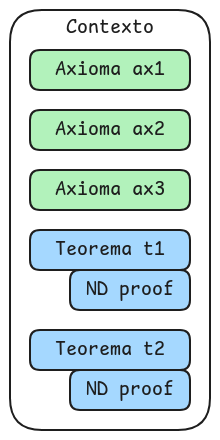
\includegraphics[scale=0.5]{img/ppa-context.png}
    \end{multicols}
    \caption{Contexto resultante de certificar de un programa}
    \label{ppa-cert:fig:context}
\end{figure}


Se puede ver un ejemplo en la \namedref{ppa-cert:fig:context}. También se puede ver
en el tipo de la función principal del módulo: \mintinline{haskell}{certify ::
Program -> Result Context}. Como para un programa generamos muchas
demostraciones, debemos extender el chequeo a contextos: Cada demostración será
válida en el \textit{prefijo estricto del contexto} que la contiene. Es decir, a
la hora de chequear la demostración de un teorema, se deben asumir como ciertas
todas las hipótesis que fueron definidas antes que él. En el ejemplo, cuando
chequeamos la demostración de \lstinline{t1}, debemos asumir como válidos los
axiomas \lstinline{ax1, ax2, ax3}.

\subsection{Contexto local}

Pero no solo los axiomas y teoremas declarados en el programa se agregan al
contexto. Cada demostración de un teorema tendrá además un \textit{contexto
local} que extiende al anterior, solo válido durante el alcance de su
demostración (se omiten en el certificado).

En él, las afirmaciones auxiliares que no afectan la tesis como
\lstinline{have}, \lstinline{claim} y \lstinline{consider}, etc. se agregan como
teoremas. Por lo tanto, cuando se citen, se pueden copiar sus demostraciones tomándolas del contexto local. Por otro
lado, algunos comandos agregan axiomas, los mismos que en deducción natural
agregan fórmulas al contexto (\lstinline{suppose} y \lstinline{consider}). Es
correcto asumir como ciertas esas hipótesis, porque lo mismo se hará durante el
chequeo de la demostración generada de deducción natural. Se puede ver un
ejemplo en la \fullref{ppa-cert:fig:local-context}.

\begin{figure}[h]
    \centering
    \begin{multicols}{2}
        \begin{tabular}{c}
            \lstinputlisting{listings/certifier/local-context.ppa}
        \end{tabular}
        \vfill\null
        \columnbreak
        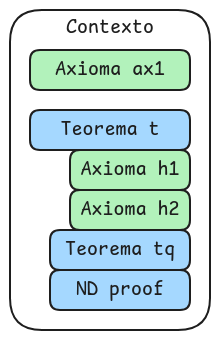
\includegraphics[scale=0.5]{img/ppa-local-context.png}
    \end{multicols}
    \caption{Contexto local}
    \label{ppa-cert:fig:local-context}
\end{figure}

\section{Certificado de demostraciones}

Ya vimos cómo las hipótesis se agregan al contexto. Pero ¿cómo generamos una demostración de deducción natural a partir de una demostración de un teorema de \ppaLang{}? Para cada comando introducido en el \namedref{chap:ppa}, deberemos \textit{certificarlo} generando una demostración, y el resto del programa debería demostrar sus premisas. En la \namedref{ppa-cert:certify:ex} se puede ver un ejemplo, en donde \lstinline{take} se certifica como \ruleExistsI{}, y la demostración de su premisa está dada por el certificado del resto del programa, \lstinline{thus p(v) by ax}, que se certifica como \ruleAx.

\begin{figure}[H]
    \begin{multicols}{2}
        \begin{tabular}{c}
            \lstinputlisting{listings/extract/exists.ppa}
        \end{tabular}
        \begin{prooftree}
            \AxiomC{}
            \RL{\ruleAx}
            \UnaryInfC{$p(v) \judG p(v)$}
            \RL{\ruleExistsI}
            \UnaryInfC{$p(v) \judG \exists x . p(X)$}
        \end{prooftree}
    \end{multicols}
    \caption{Ejemplo de certificado generado para un programa}
    \label{ppa-cert:certify:ex}
\end{figure}

En el resto del capítulo presentamos cómo cada comando de \ppaLang{} puede ser certificado.

\begin{itemize}
    \item Comenzamos con describir el \textit{solver} que se usa por debajo del \lstinline{by}, que es central al funcionamiento de todo el certificador. Aquí veremos que la demostración generada para \ref{ppa-cert:certify:ex} no es exactamente como se presenta.
    \item Vemos cómo podemos usarlo para facilitar la descarga de conjunciones en un orden arbitrario.
    \item También la traducción de los comandos que corresponden a reglas de inferencia de forma directa: \lstinline{take} (\ruleExistsI), \lstinline{consider} (\ruleExistsE), \lstinline{let} (\ruleForallI), \lstinline{cases} (\ruleOrE) y \lstinline{suppose} (\ruleImpI, \ruleNotI).
    \item Y finalmente los comandos adicionales: \lstinline{equivalently} y \lstinline{claim}.
\end{itemize}

\section{Implementación del by}

El \lstinline{by} es el mecanismo principal de demostración en PPA, y el corazón
del \modCertifier. Muchas funcionalidades están implementadas a su alrededor.
Genera \textbf{automáticamente} una demostración de que una fórmula es
consecuencia lógica de una lista de hipótesis. Es un \textit{solver heurístico} para lógica de primer orden. Está basado en la implementación del mecanismo análogo en el \texttt{Checker} de Mizar \cite{freek-by}.

Sea $A$ una fórmula. Supongamos que queremos demostrar \lstinline{thus A by h1, ..., hn} y que en el contexto tenemos que las hipótesis $h_i$ corresponden a
fórmulas $\formTwo_i$, con $i \in \{1, ..., n\}$ y $n \in \setNaturals$. Primero
veamos la idea general de la estrategia y luego profundizamos en cada paso. Los pasos para certificar un \lstinline{by} son los siguientes. 
\begin{itemize}
    \item Queremos demostrar la implicación de las hipótesis a la fórmula.
    \[
        \formTwo_1 \fAnd \dots \fAnd \formTwo_n \fImp \form
    \]
    A esta fórmula la llamamos \textbf{tesis}.
    \item \textbf{Razonamos por el absurdo}: asumiendo la negación de la tesis encontramos una contradicción
    \begin{align*}
        \fNot (\formTwo_1 \fAnd \dots \fAnd \formTwo_n \fImp \form)
        &\equiv \fNot (\fNot (\formTwo_1 \fAnd \dots \fAnd \formTwo_n) \fOr \form)\\
        &\equiv \formTwo_1 \fAnd \dots \fAnd \formTwo_n \fAnd \fNot \form
    \end{align*}
    \item Convertimos la negación de la tesis a forma normal disyuntiva (\textbf{DNF}),
    una disyunción de conjunciones de literales (``cláusulas'').
    \[
        (\formLit^1_{1} \fAnd \dots \fAnd \formLit^1_{n_1})
        \fOr \dots \fOr
        (\formLit^m_{1} \fAnd \dots \fAnd \formLit^m_{n_m})
    \]

    donde $m \in \setNaturals$ es el número de cláusulas, $n_1, \dots, n_m \in
    \setNaturals$ es la cantidad de fórmulas de cada cláusula y $\formLit^i_j$
    es la $j$-ésima fórmula de la $i$-ésima cláusula.

    \duda{Me parece que me compliqué de más con esta notación. Estaría OK dejarlo como \(
        (\formLit_1 \fAnd \dots \fAnd \formLit_n)
        \fOr \dots \fOr
        (\formLitTwo_1 \fAnd \dots \fAnd \formLitTwo_m)
    \)?}
    \item Buscamos una \textbf{contradicción} refutando cada cláusula individualmente.
    Una cláusula $\formLit_1 \fAnd \dots \fAnd \formLit_n$ será refutable si
    cumple una de las siguientes condiciones.
    \begin{itemize}
        \item Contiene $\fFalse$
        \item Contiene dos fórmulas opuestas ($\formLit, \fNot \formLit$)
        \item Eliminando existenciales consecutivos y re-convirtiendo a DNF, se
        consigue una refutación ($\fNot \pred(k), \forall \var .\ \pred(x)$)
    \end{itemize}
\end{itemize}

La complejidad del mecanismo no reside solo en tener que realizar todos estos
pasos, sino que el desafío principal fue \textbf{generar la demostración en
deducción natural}. Veamos un ejemplo sin generar la demostración, y sin
eliminar existenciales.

\begin{ejemplo}[Ejemplo sin cuantificadores]
    Tenemos el siguiente programa

    \begin{figure}[H]
        \centering
        \begin{tabular}{c}
            \lstinputlisting{listings/certifier/by-modus-ponens.ppa}
        \end{tabular}
    \end{figure}

    Para certificar \lstinline{thus b by ax1, ax2} hay que generar una
    demostración para la implicación $\big((a \fImp b) \wedge a \big)\fImp b$.

    \begin{enumerate}
        \item Negamos la fórmula 
        \[ \fNot [ \big( (a \to b) \fAnd a \big) \to b ] \]

        \item La convertimos a DNF
        \begin{align*}
            &\fNot [ \big( (a \to b) \fAnd a \big) \to b ] \\
            &\equiv \fNot [ \fNot \big( (a \to b) \fAnd a \big) \fOr b ]
                && (\form \to \formTwo \equiv \fNot \form \fOr \formTwo)\\
            &\equiv \fNot \fNot \big( (a \to b) \fAnd a \big) \fAnd \fNot b
                && (\fNot(\form \fOr \formTwo) \equiv \fNot \form \fAnd \fNot \formTwo)\\
            &\equiv \big( (a \to b) \fAnd a \big) \fAnd \fNot b
                && (\fNot\fNot \form \equiv \form)\\
            &\equiv (\fNot a \fOr b) \fAnd a \fAnd \fNot b
                 && (\form \to \formTwo \equiv \fNot \form \fOr \formTwo)\\
            &\equiv (\fNot a \fOr b) \fAnd a \fAnd \fNot b
                && ((\form \fOr \formTwo) \fAnd \formThree \equiv (\form \fAnd \formThree) \fOr (\formTwo \fAnd \formThree))\\
            &\equiv
                (\fNot a \fAnd a \fAnd \fNot b)
                \vee
                (b \fAnd a \fAnd \fNot b)
        \end{align*}

        \item Buscamos una contradicción refutando cada cláusula
        \begin{itemize}
            \item En $(\fNot a \fAnd a \fAnd \fNot b)$ tenemos $\fNot a$ y $a$.
            \item En $(b \fAnd a \fAnd \fNot b)$ tenemos $b$ y $\fNot b$.
        \end{itemize}
    \end{enumerate}
\end{ejemplo}

\subsection{Certificado del by}

En el resto de la sección, entramos en detalle de cómo generar una demostración para cada paso del by.

\begin{enumerate}
    \item \fullref{ppa-cert:sec:abs-reasoning}: primero necesitamos una forma de razonar por el absurdo, que nos permita deducir la fórmula original asumiendo su negación y demostrando $\fFalse$. Esto lo hacemos mediante dos reglas admisibles: la eliminación de doble negación (\ruleDnegE{}), equivalente a \ruleLEM{}, y \ruleCut{} que nos permite juntar demostraciones.
    \item \fullref{ppa-cert:sec:dnf}: luego vemos cómo demostrar de forma automática que una fórmula es equivalente a su versión en DNF, que se realiza a partir de un sistema de reescritura.
    \item \fullref{ppa-cert:sec:contradictions}: una vez que la fórmula está en DNF, tenemos que demostrar a partir de ella una contradicción. 
    \item \fullref{ppa:sec:by:forall-elim}: si no se encuentra una contradicción de forma simple, se procede a eliminar $\forall$ consecutivos y reiniciar el proceso pero con unificación de fórmulas en lugar de igualdad, para así instanciar las variables cuantificadas universalmente.
    \item \fullref{ppa-cert:sec:expressiveness}: finalmente evaluamos el poder expresivo del \textit{solver} implementado, que resulta completo para proposicional y heurístico para primer orden.
\end{enumerate}


\subsection{Razonamiento por el absurdo}
\label{ppa-cert:sec:abs-reasoning}

Queremos asumir que no vale la fórmula original, es decir $\fNot (\formTwo_1
\fAnd \dots \fAnd \formTwo_n \fImp \form)$, y llegar a una contradicción. Pero
en la demostración que estamos generando, tenemos que demostrar $(\formTwo_1
\fAnd \dots \fAnd \formTwo_n \fImp \form)$. ¿Cómo se puede razonar por el
absurdo?

De la misma forma que en la \namedref{nd:sec:admissible-rules} se introduce
\textit{modus tollens} como una regla admisible, para razonar por el absurdo
vamos a usar la \textbf{eliminación de la doble negación}. Es un principio de
razonamiento clásico que es equivalente a LEM.


\begin{theorem}[Eliminación de la doble negación]
    Sea $\form$ una fórmula cualquiera. Vale $\fNot \fNot \form \judG \form$, y lo notamos como regla admisible

    \begin{prooftree}
        \AxiomC{}
        \RL{\ruleDnegE}
        \admissibleRuleLine
        \UnaryInfC{$\fNot \fNot \form \judG \form$}
    \end{prooftree}
\end{theorem}
\begin{proof}
    En deducción natural,

    \begin{prooftree}
        \def\defaultHypSeparation{\hskip .1in} % default .2in
        \AxiomC{}
        \LL{\ruleLEM}
        \UnaryInfC{$\fNot \fNot \form \judG \form \fOr \fNot \form$}
        \AxiomC{}
        \RL{\ruleAx}
        \UnaryInfC{\(
            \fNot \fNot \form, \form \judG \form
        \)}
        \AxiomC{}
        \LL{\ruleAx}
        \UnaryInfC{\(
            \fNot \fNot \form, \fNot\form \judG \fNot \fNot \form
        \)}
        \AxiomC{}
        \RL{\ruleAx}
        \UnaryInfC{\(
            \fNot \fNot \form, \fNot\form \judG \fNot \form
        \)}
        \RL{\ruleNotE}
        \BinaryInfC{\(
            \fNot \fNot \form, \fNot \form \judG \form
        \)}
        \RL{\ruleOrE}
        \TrinaryInfC{$\fNot \fNot \form \judG \form$}
    \end{prooftree}
\end{proof}

¿Cómo lo usamos? Introducimos otra regla admisible: \textbf{cut}, que nos
permite ``pegar'' demostraciones entre sí. Si estamos queriendo demostrar
$\form$, y queremos reducir el problema a $\formTwo$ que sí podemos probar, esta
regla nos permite hacerlo.

\begin{theorem}[Cut] La siguiente regla de inferencia es admisible
\begin{prooftree}
    \AxiomC{$\ctx, \formTwo \judG \form$}
    \AxiomC{$\ctx \judG \formTwo$}
    \RL{\ruleCut}
    \admissibleRuleLine
    \BinaryInfC{$\ctx \judG \form$}
\end{prooftree}
\end{theorem}

\begin{proof}
    La regla \ruleCut{} se puede ver como un \textit{macro} que por atrás genera
    la siguiente demostración
    
    \begin{prooftree}
        \AxiomC{$\ctx, \formTwo \judG \form$}
        \RL{\ruleImpI}
        \UnaryInfC{$\ctx \judG \formTwo \fImp \form$}
        \AxiomC{$\ctx \judG \formTwo$}
        \RL{\ruleImpE}
        \BinaryInfC{$\ctx \judG \form$}
    \end{prooftree}
\end{proof}

\begin{ejemplo}
Cut nos permite continuar la demostración por otra fórmula a partir de la cual
podamos demostrar la original. Sean $\someProof_{\formTwo \fImp \form}$ una
demostración de $\formTwo \judG \form$ y $\someProof_\formTwo$ una demostración
de $\formTwo$ (la continuación). Podemos usar cut de la siguiente manera.

\begin{prooftree}
    \AxiomC{$\someProof_{\formTwo \fImp \form}$}
    \noLine
    \UnaryInfC{$\ctx, \formTwo \judG \form$}
    \AxiomC{$\someProof_\formTwo$}
    \noLine
    \UnaryInfC{$\ctx \judG \formTwo$}
    \RL{\ruleCut}
    \admissibleRuleLine
    \BinaryInfC{$\ctx \judG \form$}
\end{prooftree}

Que es certificado como

\begin{prooftree}
    \AxiomC{$\someProof_{\formTwo \fImp \form}$}
    \noLine
    \UnaryInfC{$\ctx, \formTwo \judG \form$}
    \RL{\ruleImpI}
    \UnaryInfC{$\ctx \judG \formTwo \fImp \form$}
    \AxiomC{$\someProof_\formTwo$}
    \noLine
    \UnaryInfC{$\ctx \judG \formTwo$}
    \RL{\ruleImpE}
    \BinaryInfC{$\ctx \judG \form$}
\end{prooftree}
\end{ejemplo}


\begin{notation*}
    En los casos en donde queramos continuar la demostración por la nueva y la demostración de la implicación sea omitida (por ejemplo por ser una regla admisible) lo notaremos de una forma más sucinta:

    \begin{prooftree}
        \AxiomC{$\someProof_\formTwo$}
        \noLine
        \UnaryInfC{$\ctx \judG \formTwo$}
        \RL{\ruleCutWith{$\someProof_{\formTwo \fImp \form}$}}
        \admissibleRuleLine
        \UnaryInfC{$\ctx \judG \form$}
    \end{prooftree}
\end{notation*}

\begin{lemma}[Razonamiento por el absurdo]
    \label{ppa:sec:abs-reasoning}
    Imaginemos que queremos demostrar
$\form$ por el absurdo. Podemos juntar con cut con la eliminación de la doble
negación, pasando a demostrar $\fNot \fNot \form$. Al introducirla,
debemos demostrar el juicio $\ctx, \fNot \form \judG \fFalse$:
asumiendo que no es cierta la fórmula, deducimos una contradicción.

\begin{prooftree}
    \AxiomC{}
    \RL{\ruleDnegE}
    \admissibleRuleLine
    \UnaryInfC{$\ctx, \fNot \fNot \form \judG \form$}
    \AxiomC{$\vdots$}
    \noLine
    \UnaryInfC{$\ctx, \fNot \form \judG \fFalse$}
    \RL{\ruleNotI}
    \UnaryInfC{$\ctx \judG \fNot\fNot \form$}
    \RL{\ruleCut}
    \admissibleRuleLine
    \BinaryInfC{$\ctx \judG \form$}
\end{prooftree}

Que también se puede notar de la siguiente forma

\begin{prooftree}
    \AxiomC{$\vdots$}
    \noLine
    \UnaryInfC{$\ctx, \fNot \form \judG \fFalse$}
    \RL{\ruleNotI}
    \UnaryInfC{$\ctx \judG \fNot\fNot \form$}
    \RL{\ruleCutWith{\ruleDnegE}}
    \admissibleRuleLine
    \UnaryInfC{$\ctx \judG \form$}
\end{prooftree}

\end{lemma}

\begin{obs*}
    A \ruleDnegE{} La formulamos como $\fNot \fNot \form \judG \form$ y la usamos con
    \textbf{cut}, pero otra alternativa equivalente, levemente más tediosa para
    generar demostraciones, hubiera sido demostrarla como $\fNot \fNot \form
    \fImp \form$ y usarla con \ruleImpE{} directamente.
\end{obs*}

\subsection{Conversión a DNF}
\label{ppa-cert:sec:dnf}

Tenemos que generar una demostración de que la negación de la tesis genera una
contradicción, pero lo queremos hacer a partir de la tesis en DNF. ¿Cómo la convertimos?. Más aún, ¿Cómo generamos una demostración para la conversión?.

\begin{definition}[DNF]
    Una fórmula está en \textbf{forma normal disyuntiva} o DNF
    (\textit{disjunctive normal form}) si es una disyunción de conjunciones de
    literales.  Llamamos \textbf{cláusulas} a las conjunciones que la
    componen. Un literal será un predicado, una negación de un predicado o una
    fórmula cualquiera que comienza con un cuantificador. Ejemplos:
    
    Sean $\formLit, \formLitTwo, \formLitThree$ predicados 0-arios. Luego,
    \begin{itemize}
        \item $\formLit \fAnd \formLitTwo$ está en DNF.
        \item $(\formLit \fAnd \formLitThree) \fOr (\formLit \fAnd \formLitTwo)$ también.
        \item $(\formLit \fImp \formLitTwo) \fOr (\formLit \fAnd \formLitTwo)$ no lo está.
        \item $\big(\forall \var . (\formLit \fImp \formLitTwo)\big) \fOr (\formLit \fAnd \formLitTwo)$ si.
    \end{itemize}
\end{definition}

\begin{theorem}[Conversión a DNF]
    \label{ppa-cert:thm:dnf}
    
    Para toda fórmula $\form$, existe
    $\dnf{\form}$ su equivalente en DNF. Y vale $\form \judG \dnf{\form}$.
\end{theorem}

\begin{obs}
    Continuamos la demostración por la refutación de la fórmula en DNF mediante
el uso de cut.

\begin{prooftree}
    \AxiomC{\vdots}
    \noLine
    \UnaryInfC{$\ctx, \form \judG \dnf{\form}$}
    \AxiomC{\vdots}
    \noLine
    \UnaryInfC{$\ctx, \form, \dnf{\form} \judG \fFalse$}
    \RL{\ruleCut}
    \admissibleRuleLine
    \BinaryInfC{$\ctx, \form \judG \fFalse$}
\end{prooftree}
\end{obs}


Para convertir una fórmula cualquiera a DNF, vamos a implementar una traducción
\textit{small-step} mediante el siguiente sistema de reescritura.

\begin{figure}[H]
    \begin{align*}
        \fNot\fNot \formLit &\rewrite
            \formLit
            &&\text{eliminación de $\fNot\fNot$}\\
        \fNot \fFalse &\rewrite
            \fTrue\\
        \fNot \fTrue &\rewrite
            \fFalse\\
        \formLit \fImp \formLitTwo &\rewrite
            \fNot \formLit \fOr \formLitTwo
            &&\text{definición de implicación}\\
        \fNot(\formLit \fOr \formLitTwo) &\rewrite
            \fNot \formLit \fAnd \fNot \formLitTwo
            &&\text{distributiva de $\fNot$ sobre $\fAnd$}\\
        \fNot(\formLit \fAnd \formLitTwo) &\rewrite
            \fNot \formLit \fOr \fNot \formLitTwo
            &&\text{distributiva de $\fNot$ sobre $\fOr$}\\
        (\formLit \fOr \formLitTwo) \fAnd \formLitThree &\rewrite
            (\formLit \fAnd \formLitThree) \fOr (\formLitTwo \fAnd \formLitThree)
            &&\text{distributiva de $\fAnd$ sobre $\fOr$ (der)}\\
        \formLitThree \fAnd (\formLit \fOr \formLitTwo) &\rewrite
            (\formLitThree \fAnd \formLit) \fOr (\formLitThree \fAnd \formLitTwo)
            &&\text{distributiva de $\fAnd$ sobre $\fOr$ (izq)}\\
        \formLit \fOr (\formLitTwo \fOr \formLitThree) &\rewrite
            (\formLit \fOr \formLitTwo) \fOr \formLitThree
            &&\text{asociatividad de $\fOr$}\\
        \formLit \fAnd (\formLitTwo \fAnd \formLitThree) &\rewrite
            (\formLit \fAnd \formLitTwo) \fAnd \formLitThree
            &&\text{asociatividad de $\fAnd$}
    \end{align*}    
    \caption{Sistema de reescritura para conversión a DNF de forma sintáctica}
\end{figure}

Pero no podemos hacerlo meramente de forma sintáctica, sino que tenemos
\textit{generar una demostración} para cada equivalencia. Cada una será una regla admisible.

\subsubsection{Congruencias}

Hay pasos de la traducción a DNF en donde tenemos que reemplazar una sub-fórmula por una equivalente.  Por ejemplo para reescribir
\(
    \formLit \fOr \bm{\fNot (\formLitTwo \fOr \formLitThree)}
    \rewrite
    \formLit \fOr \bm{(\fNot \formLitTwo \fAnd \fNot \formLitThree)}
\)
reescribimos la sub-fórmula $\fNot
(\formLitTwo \fOr
\formLitThree) \rewrite \fNot \formLitTwo \fAnd \fNot \formLitThree$.
Esto de forma sintáctica sería trivial, basta con hacerlo recursivamente. Pero para demostrarlo hay que usar la la
\textit{congruencia} de los conectivos, que también hay que demostrar.
\begin{align*}
    \form \judG \form'
        &\Rightarrow \form \fAnd \formTwo \judG \form' \fAnd \formTwo\\
    \form \judG \form'
        &\Rightarrow \form \fOr \formTwo \judG \form' \fOr \formTwo\\
    \form' \judG \form
        &\Rightarrow \fNot \form \judG \fNot \form'
\end{align*}
No hay regla de congruencia para $\fImp$ pues se convierte en un $\fOr$. Es
sumamente importante observar que $\fNot$ es \textit{contravariante}, para
demostrar $\fNot \form \judG \fNot \form'$ no necesitamos una demostración
de $\form \judG \form'$, sino de $\form' \judG \form$. Esto quiere decir que
para todas las equivalencias, incluso las congruencias, no nos alcanza con
demostrarlas en un solo sentido, ya que si se usan dentro de un $\fNot$, necesitaremos el otro. Vamos a necesitar demostrar la
ida y la vuelta: para $\fNot(\formLit \fOr \formLitTwo) \rewrite
\fNot \formLit \fAnd \fNot \formLitTwo$ necesitamos
\(
    \fNot(\formLit \fOr \formLitTwo)
        \judG \fNot \formLit \fAnd \fNot \formLitTwo
\) y \(
    \fNot \formLit \fAnd \fNot \formLitTwo \judG \fNot(\formLit \fOr \formLitTwo)
\). Lo notamos como \[
    \fNot(\formLit \fOr \formLitTwo)
        \judgEquiv \fNot \formLit \fAnd \fNot \formLitTwo
\]

\subsubsection{Algoritmo}
\label{ppa:sec:dnf:algoritmo}

Finalmente, el algoritmo para generar la demostración de la conversión de una
fórmula en DNF se implementa en dos partes. Por un lado, contamos con una
conversión \textit{small-step} que hace un paso de reescritura. Con él, podemos
implementar la conversión como su \textit{clausura reflexiva transitiva}:
aplicarla 0 o más veces hasta que ya no cambie. Los pasos pueden ser o bien ser
un paso de reescritura, o muchos recursivos de congruencia para reescribir una sub-fórmula anidada. En cada uno se usa una de las demostraciones de la \namedref{ppa-cert:dnf-rules}. En total son 26 demostraciones. Nos ahorramos los detalles porque son sencillas y bien conocidas, por ejemplo leyes de De Morgan.
\begin{figure}[H]
    \begin{align*}
        \intertext{Pasos base}
        \fNot\fNot \formLit &\judgEquiv
            \formLit
            \\
        \fNot \fFalse &\judgEquiv
            \fTrue\\
        \fNot \fTrue &\judgEquiv
            \fFalse\\
        \formLit \fImp \formLitTwo &\judgEquiv
            \fNot \formLit \fOr \formLitTwo
            \\
        \fNot(\formLit \fOr \formLitTwo) &\judgEquiv
            \fNot \formLit \fAnd \fNot \formLitTwo
            \\
        \fNot(\formLit \fAnd \formLitTwo) &\judgEquiv
            \fNot \formLit \fOr \fNot \formLitTwo
            \\
        (\formLit \fOr \formLitTwo) \fAnd \formLitThree &\judgEquiv
            (\formLit \fAnd \formLitThree) \fOr (\formLitTwo \fAnd \formLitThree)
            \\
        \formLitThree \fAnd (\formLit \fOr \formLitTwo) &\judgEquiv
            (\formLitThree \fAnd \formLit) \fOr (\formLitThree \fAnd \formLitTwo)
            \\
        \formLit \fOr (\formLitTwo \fOr \formLitThree) &\judgEquiv
            (\formLit \fOr \formLitTwo) \fOr \formLitThree
            \\
        \formLit \fAnd (\formLitTwo \fAnd \formLitThree) &\judgEquiv
            (\formLit \fAnd \formLitTwo) \fAnd \formLitThree\\
        \intertext{Pasos recursivos de congruencia (con $\form \judgEquiv \form'$)}
        \form \fAnd \formTwo &\judgEquiv \form' \fAnd \formTwo\\
        \form \fOr \formTwo &\judgEquiv \form' \fOr \formTwo\\
        \fNot \form &\judgEquiv \fNot \form'
    \end{align*}
    \caption{Reglas de conversión a DNF}
    \label{ppa-cert:dnf-rules}
\end{figure}

\duda{Demostración de que termina? De que es correcto? Al menos una cita para que sea más confiable el sistema de reescritura? O se asume como bien conocido?}

\subsection{Contradicciones}
\label{ppa-cert:sec:contradictions}

Tenemos la fórmula traducida a DNF. Debemos demostrar una contradicción a partir
de ella. Si tenemos las cláusulas $\clause_1 \fOr \clause_2$, podemos demostrar
$\clause_1 \fOr \clause_2 \judG \fFalse$ usando \ruleOrE{} y deducir una contradicción asumiendo cada una. Esto se generaliza a N cláusulas mediante el
uso de \ruleOrE{} anidados. Por lo tanto hay que \textit{``refutar cada
cláusula''}. El método lo hace de tres formas distintas

\begin{itemize}
    \item Contienen fórmulas opuestas: $\form \fAnd \fNot \form$ (con
    \ruleNotE{})
    \item Contienen $\fFalse$
    \item Eliminando cuantificadores universales consecutivos (\namedref{ppa:sec:by:forall-elim})
\end{itemize}

Para los primeros dos, es necesario demostrar a partir de la cláusula una
fórmula. Pero como pueden tener una cantidad arbitraria, según cómo esté
asociado el $\fAnd$, una demostración a mano de
\(
    \form_1 \fAnd \dots \fAnd \form_i \fAnd \dots \fAnd \form_n \judG \form_i,
\)
puede ser muy laboriosa, dado que las reglas son binarias y habría que usar
\ruleAndEOne{} y \ruleAndETwo{} anidados. Para simplificarlo demostramos otra
regla admisible, la proyección de un elemento \ruleAndEProj{\anyForm}.

\begin{theorem}[Regla admisible \ruleAndEProj{\anyForm}]
    Sea $\anyForm$ alguna fórmula de la conjunción $\anyForm_1 \fAnd \dots \fAnd
    \anyForm_n$. Notamos por \ruleAndEProj{\anyForm} a la proyección \textit{de
    la fórmula}, sin importar en qué posición de la conjunción está.

    \begin{prooftree}
        \AxiomC{$\ctx \judG \anyForm_1 \fAnd \dots \fAnd \anyForm_i \fAnd \dots \fAnd \anyForm_n$}
        \AxiomC{$n \in \setNaturals$}
        \admissibleRuleLine
        \RL{\ruleAndEProj{\anyForm_{i}}}
        \BinaryInfC{$\ctx \judG \anyForm_i$}
    \end{prooftree}
\end{theorem}
\begin{proof}
    Para generar la demostración correspondiente usando \ruleAndEOne{} y
    \ruleAndETwo{}, basta con identificar el camino hacia $\anyForm_i$, y luego
    caminar recursivamente el $\fAnd$ usando \ruleAndEOne{} si el camino
    continúa por la izquierda y \ruleAndETwo{} si sigue por la derecha.
\end{proof}

\begin{ejemplo}[Contradicción]
    Veamos un ejemplo de las primeras dos formas de refutar cláusulas. Los
    cuantificadores universales los veremos en la siguiente sección.
\begin{prooftree}
    \AxiomC{}
    \LL{\ruleAx}
    \UnaryInfC{\(
        \ctx \judG (\fNot a \fAnd a \fAnd \fNot b)\vee (b \fAnd a \fAnd \fFalse)
    \)}
    \AxiomC{$\someProof_L$}
    \noLine
    \UnaryInfC{\(
        \ctx, \fNot a \fAnd a \fAnd \fNot b \judG \fFalse
    \)}
    \AxiomC{}
    \RL{\ruleAx}
    \UnaryInfC{$\ctx_1 \judG b \fAnd a \fAnd \fFalse$}
    \RL{\ruleAndEProj{\fFalse}}
    \admissibleRuleLine
    \UnaryInfC{\(
        \ctx, b \fAnd a \fAnd \fFalse \judG \fFalse
    \)}
    \RL{\ruleOrE}
    \TrinaryInfC{\(
        \ctx = (\fNot a \fAnd a \fAnd \fNot b)
        \vee
        (b \fAnd a \fAnd \fFalse)
        \judG
        \fFalse
    \)}
\end{prooftree}

donde

\begin{prooftree}
    \AxiomC{}
    \RL{\ruleAx}
    \UnaryInfC{$\ctx_1 \judG \fNot a \fAnd a \fAnd \fNot b$}
    \RL{\ruleAndEProj{\fNot a}}
    \admissibleRuleLine
    \UnaryInfC{$\ctx_1 \judG \fNot a$}
    \AxiomC{}
    \RL{\ruleAx}
    \UnaryInfC{$\ctx_1 \judG \fNot a \fAnd a \fAnd \fNot b$}
    \RL{\ruleAndEProj{a}}
    \admissibleRuleLine
    \UnaryInfC{$\ctx_1 \judG a$}
    \RL{\ruleNotE}
    \LL{$\someProof_L=$}
    \BinaryInfC{\(
        \ctx_1 = \ctx, b \fAnd a \fAnd \fFalse \judG \fFalse
    \)}
\end{prooftree}
\end{ejemplo}

\duda{No se si me convence la notación \ruleAndEProj{\alpha}, después de todo es
una proyección y se suele notar con $\Pi$, pero ese símbolo lo estamos usando
para representar demostraciones (ej. $\someProof_L$).}

\subsection{Eliminación de cuantificadores universales}
\label{ppa:sec:by:forall-elim}

Hasta ahora logramos razonar por el absurdo, convertir la fórmula a DNF, y
encontrar una contradicción siempre que no haya que eliminar cuantificadores
universales. Pero es usual que en una teoría de primer orden, los axiomas los
usen y sea necesario eliminarlos para poder demostrar un \lstinline{by}. Al
hacerlo, vamos a reemplazar las ocurrencias de su variable por
\textit{meta-variables}: aquellas que pueden ser unificadas.
    
\begin{definition}[Unificación]
    Sean $\form$, $\formTwo$ dos fórmulas. Decimos que \textit{unifican} y lo
    notamos $\form \unify \formTwo$ si existe una sustitución de
    meta-variables tal que $\form = \formTwo$. Veamos algunos ejemplos. Sean $\metavar{u}, \metavar{v}$ meta-variables.

    \begin{itemize}
    \item $p(\metavar{u}) \unify p(a)$ con $\subst{\metavar{u}}{a}$
        \item $p(\metavar{u}) \not\unify q(a)$
        \item $p(\metavar{u}) \fAnd q(b) \unify p(a) \fAnd q(\metavar{v})$
        con $\substTwo{\metavar{u}}{a}{\metavar{v}}{b}$
        \item $p(\metavar{u}) \fImp q(b) \not\unify p(a) \fAnd q(\metavar{v})$
    \end{itemize}
    
    \duda{Hace falta agregar el algoritmo de unificación que implementamos?}
\end{definition}

\begin{ejemplo}[Ejemplo de by con cuantificadores]
    Tenemos el siguiente programa

    \begin{figure}[H]
        \centering
        \begin{tabular}{c}
            \lstinputlisting{listings/certifier/by-modus-ponens-quant.ppa}
        \end{tabular}
    \end{figure}

    Para certificar \lstinline{thus q(a) by ax1, ax2} hay que generar una
    demostración para la implicación \(
        \Big(\big(\forall x. (p(x) \fImp q(x))\big) \fAnd p(a) \Big)
        \fImp q(a)
    \).

    \begin{enumerate}
        \item Negamos la fórmula 
        \[
            \fNot \left[
            \Big(\big(\forall x. (p(x) \fImp q(x))\big) \fAnd p(a) \Big)
            \fImp q(a)
        \right].
        \]

        \item La convertimos a DNF
        \begin{align*}
            &\fNot \left[
                \Big(\big(\forall x. (p(x) \fImp q(x))\big) \fAnd p(a) \Big)
                \fImp q(a)
            \right] \\
            &\equiv \fNot \left[
                \fNot \Big(\big(\forall x. (p(x) \fImp q(x))\big) \fAnd p(a) \Big)
                \fOr q(a)
            \right] 
                && (\form \to \formTwo \equiv \fNot \form \fOr \formTwo)\\
            &\equiv
                \fNot \fNot \Big(\big(\forall x. (p(x) \fImp q(x))\big) \fAnd p(a) \Big)
                \fAnd \fNot q(a)
                && (\fNot(\form \fOr \formTwo) \equiv \fNot \form \fAnd \fNot \formTwo)\\
            &\equiv \big(\forall x. (p(x) \fImp q(x))\big) \fAnd p(a)
            \fAnd \fNot q(a)
                && (\fNot\fNot \form \equiv \form)
        \end{align*}

        como a los ojos de DNF un $\forall$ es opaco, a pesar de que dentro
        tenga una implicación, la fórmula ya está en forma normal.

        \item Buscamos una contradicción refutando cada cláusula. No hay forma
        encontrando literales opuestos o $\fFalse$, por ej. la cláusula
        $p(a)$ no es refutable.
        \item Probamos eliminando $\forall x. (p(x) \fImp q(x))$. Reemplazamos
        $x$ por una meta-variable fresca $\metavar{u}$.
        \[
            (p(\metavar{u}) \fImp q(\metavar{u})) \fAnd p(a) \fAnd \fNot q(a)
        \]
        ¡No está en DNF! Hay que volver a convertir.
        \item Convertimos a DNF
        \begin{align*}
            &(p(\metavar{u}) \fImp q(\metavar{u})) \fAnd p(a) \fAnd \fNot q(a)\\
            &\equiv (\fNot p(\metavar{u}) \fOr q(\metavar{u})) \fAnd p(a) \fAnd \fNot q(a)
            &&(\form \to \formTwo \equiv \fNot \form \fOr \formTwo)\\
            &\equiv ( (\fNot p(\metavar{u}) \fAnd p(a)) \fOr (q(\metavar{u}) \fAnd p(a))) \fAnd \fNot q(a)
            &&((\form \fOr \formTwo) \fAnd \formThree \equiv (\form \fAnd \formThree) \fOr (\form \fAnd \formThree))\\
            &\equiv 
            \begin{aligned}[t]
                &(\fNot p(\metavar{u}) \fAnd p(a) \fAnd \fNot q(a))\ \fOr\\
                &(q(\metavar{u}) \fAnd p(a)\fAnd \fNot q(a))
            \end{aligned}
            &&((\form \fOr \formTwo) \fAnd \formThree \equiv (\form \fAnd \formThree) \fOr (\form \fAnd \formThree))
        \end{align*}
        \item Buscamos una contradicción refutando cada cláusula. Esta vez, no
        podemos volver a eliminar un forall (por motivos de eficiencia) y los
        literales opuestos tienen que \textit{unificar} en lugar de ser iguales.
        Las sustituciones tienen que ser compatibles entre todas las cláusulas
        (no pueden asignar valores diferentes a la misma meta-variable)
        \begin{itemize}
            \item $\fNot p(\metavar{u}) \fAnd p(a) \fAnd \fNot q(a)$ tenemos $p(\metavar{u}) \unify p(a)$ con $\subst{\metavar{u}}{a}$
            \item $q(\metavar{u}) \fAnd p(a) \fAnd \fNot q(a)$ tenemos $q(\metavar{u}) \unify q(a)$ con $\subst{\metavar{u}}{a}$
        \end{itemize}
    \end{enumerate}
\end{ejemplo}

\subsubsection{Algoritmo}
\begin{enumerate}
    \item Si la cláusula no puede ser refutada por contener $\fFalse$ ni literales opuestos,
    \item Para cada fórmula, si comienza con $\forall$ (ej. $\forall \var_0 . \forall x_1 \dots \forall \var_n . p(\var_0, \dots, \var_n)$) se busca una refutación sin generar la demostración.
    \begin{itemize}
        \item Para cada combinación de prefijos de $\forall$ consecutivos, se
        reemplazan sus variables por meta-variables frescas, se re-convierte a
        DNF y se intenta encontrar una refutación (unificando con $\alpha-$equivalencia)
        \begin{itemize}
            \item $\forall \var_1 \dots \forall \var_n . p(u_0, \dots, \var_n)$
            \item $\dotso$
            \item $p(u_0, \dots, u_n)$
        \end{itemize}
        \item Se usa la menor cantidad de eliminaciones posibles.
        \item Si puede ser refutada, nos da como resultado una sustitución que asigna a cada meta-variable $u_i$ un término $t_i$.
    \end{itemize}
    \item Se usa \ruleForallE{} reemplazando cada variable por el término asignado a la meta-variable correspondiente, para obtener la fórmula con los $\forall$ eliminados, y luego se genera la demostración de la refutación de la forma usual.
\end{enumerate}

\begin{ejemplo}[Eliminación consecutiva minimal]
Si se tiene
\[
    (\forall x. \forall y . p(x) \fOr q(y)) \fAnd \fNot p(a) \fAnd \fNot q(b)
\]

se reemplazarían tanto $x$ como $y$ por meta-variables frescas $u_0$ y $u_1$, quedando así $(p(u_0) \fOr q(u_1)) \fAnd \fNot p(a) \fAnd \fNot q(b)$ que se podrá refutar. En cambio, en
\[
    (\forall x. \forall y . p(x) \fAnd q(y)) \fAnd \fNot (\forall z. p(a) \fAnd q(z))
\]

es necesario eliminar solamente $\forall x$. Y la unificación será capaz de tener en cuenta la alpha equivalencia, así puede unificar $\forall y . p(u_0) \fAnd q(y) \unify \forall z. p(a) \fAnd q(z)$.
\end{ejemplo}

\begin{ejemplo}[Eliminación de una sola fórmula]
    Se eliminan los $\forall$ consecutivos de una sola fórmula de la cláusula. Por ejemplo, en la siguiente o bien eliminamos $\forall x . p(x)$ o $\forall y . q(y)$ pero no ambos.
\[
    (\forall x . p(x)) \fAnd (\forall y . q(y)) \fAnd \fNot p(a) \fAnd \fNot q(b)
\]
\end{ejemplo}


\subsubsection{Compatibilidad de sustituciones}

Como cada cláusula se refuta por separado, hay que asegurar que las sustituciones de cada una sean compatibles entre sí. Es decir, que no asignen términos diferentes a las mismas meta-variables. Debemos probar con todas las sustituciones posibles, porque puede haber algunas combinaciones incompatibles y otras no. Por ejemplo, en las siguientes cláusulas hay más de una sustitución candidata para cada una.

\begin{itemize}
    \item $f(u_0) \fAnd \fNot f(a) \fAnd \fNot f(b)$ tenemos $\subst{u_0}{a}$, $\subst{u_0}{b}$
    \item $f(u_0) \fAnd \fNot f(b)$ solo $\subst{u_0}{b}$
\end{itemize}

Pero si en la primera nos quedamos con $\subst{u_0}{a}$, no podríamos refutar la 2da. Por lo tanto la correcta es $\subst{u_0}{b}$.

\subsection{Poder expresivo}
\label{ppa-cert:sec:expressiveness}

\duda{Está bien decir poder expresivo?}

El solver implementado es \textbf{completo para lógica proposicional}, pero heurístico para lógica de primer orden. Esto es aceptable, puesto que la satisfacibilidad de lógica de primer orden es indecidible (por el teorema de Church \cite{church}), y el objetivo del trabajo no fue dar un solver innovador, sino alguno que se pueda certificar.

\begin{theorem}
    El solver es \textbf{completo} para lógica proposicional. Sea $\anyForm$ una fórmula cualquiera. Si es universalmente válida, $\judG \anyForm$, entonces el solver encuentra una demostración.
\end{theorem}
\begin{proof}
    \duda{Citar Hilbert 1950?}
Lo hacemos semánticamente. Sea $\anyForm$ una fórmula proposicional cualquiera, supongamos que es válida. Queremos argumentar que el solver va a poder generar una demostración para ello. Sabemos que es válida si y solo si su negación es insatisfactible

\[\judG \anyForm \iff \not\judG \fNot \anyForm,\]
por lo que es correcto buscar una refutación de la negación. Además, siempre vamos a poder convertir $\fNot \anyForm$ a DNF (\namedref{ppa-cert:thm:dnf}), por lo que tenemos
\[
    \not\judG\fNot \anyForm \iff
    \not\judG (\formLit_1 \fAnd \dots \fAnd \formLit_n)
    \fOr \dots \fOr
    (\formLitTwo_1 \fAnd \dots \fAnd \formLitTwo_m).
\]
Para que sea insatisfactible, por definición de la semántica de $\fOr$ todas las
cláusulas tienen que serlo. Para que una claúsula lo sea, no tiene que haber una
valuación que la haga verdadera. Supongamos que existe una valuación
$v$ que satisface $a_1 \fAnd \dots \fAnd a_n$. Está unívocamente determinada: al ser una conjunción, tiene
que asignar a cada literal $a_i$ un 1 si es positivo o un 0 si es negativo. Luego, no será verdadera si y solo si aparece la misma variable y su opuesta, o si aparece $\fFalse$. Como esto es exactamente lo que busca el solver, concluimos que si es refutable, siempre va a poder refutarla.
Por lo tanto es completo para lógica proposicional.

\duda{Está suficientemente bien escrito esto? Supongo que no. En la intro hay que agregar las definiciones de la semántica de LPO? Solo se usan acá}
\end{proof}

\begin{theorem}
    El solver es \textbf{incompleto} para lógica de primer orden.
\end{theorem}
\begin{proof}
El siguiente es un contra ejemplo, que no encuentra la refutación porque para
ello debería eliminar ambos $\forall$, pero elimina a lo sumo los de una
fórmula.
\begin{lstlisting}
axiom ax1: forall X . p(X) -> q(X)
axiom ax2: forall X . p(X)
theorem t: q(a)
proof
    thus q(a) by ax1, ax2
end
\end{lstlisting}

Pero esto no es lo único que le falta para ser completo. También se podría dar un contra ejemplo más burdo que requiera un \textit{SAT solver} completo.
\end{proof}

\subsection{Azúcar sintáctico}

La última parte de la certificación del \lstinline{by} es su azúcar sintáctico. Antes mencionamos que se puede usar \lstinline{hence} en lugar de \lstinline{thus} referenciando automáticamente a la hipótesis anterior, y análogamente lo mismo para \lstinline{have} y \lstinline{then}. Esto se implementa desde el \textit{parser}. Son solamente una construcción sintáctica que se genera directamente como \lstinline{have} o \lstinline{thus}, y se agrega la hipótesis anterior (\lstinline{-}) a cada uno. Esto simplifica al certificador, permitiendo que solo opere con ellos dos.

\section{Descarga de conjunciones}

Veamos la certificación de la \textit{descarga de conjunciones}: si la tesis es una conjunción \lstinline{a_1 & ... & a_n}, debemos poder \textit{descargar cualquier subconjunto} de ella con el \lstinline{thus}. Por ejemplo ¿cómo podemos certificar el siguiente programa?

\lstinputlisting{listings/interfaz/discharge-complex.ppa}

Veamos en particular el primer comando de la demostración. La tesis es una conjunción que está asociada de una forma particular, y se quiere demostrar $a \fAnd e$ que es parte de la tesis.

\begin{enumerate}
    \item Se convierte la conjunción y lo que se demuestra en conjuntos
    \begin{align*}
        (a \fAnd b) \fAnd ((c \fAnd d) \fAnd e)
        &\rewrite
        \{a, b, c, d, e\}\\
        (a \fAnd e) &\rewrite \{a, e\}
    \end{align*}
    \item Si está contenido, se separa lo demostrado y el resto
    \[
        \{a, b, c, d, e\} \rewrite \{b, c, d\} \{a, e\}
    \]
    \item Se construye una \textit{nueva tesis} reordenando la fórmula de forma tal que sea sencillo hacer \ruleAndI{} (poniendo a la izquierda lo demostrado aislado de lo demás)
    \[
        (a \fAnd e) \fAnd (b \fAnd c \fAnd d)
    \]

    De esa forma, al usar la regla

    \proofTreeAndI

    la demostración de $a \fAnd e$ se hace de la forma usual con by, y se reduce
    la tesis a $b \fAnd c \fAnd d$ continuando la certificación por allí,
    insertando la demostración resultante en $\ctx \judG \formTwo$.

    \item Para demostrar la equivalencia entre la tesis vieja y su versión re-ordenada se usa el mismo solver que el by. Al ser completo para proposicional, también puede resolver equivalencias por asociatividad y re-orden.
\end{enumerate}

Finalmente, queda certificado como

\begin{prooftree}
    \AxiomC{}
    \LL{solver}
    \admissibleRuleLine
    % \UnaryInfC{\shortstack{
    %     $\ctx \judG (a \fAnd e) \fAnd (b \fAnd c \fAnd d)$
    %     \\
    %     \quad$\fImp (a \fAnd b) \fAnd ((c \fAnd d) \fAnd e)$
    % }}
    \UnaryInfC{\(\begin{aligned}
        \ctx &\judG (a \fAnd e) \fAnd (b \fAnd c \fAnd d)
        \\
        &\fImp (a \fAnd b) \fAnd ((c \fAnd d) \fAnd e)
    \end{aligned}\)
    }
    \AxiomC{}
    \RL{by}
    \admissibleRuleLine
    \UnaryInfC{$\ctx \judG a \fAnd e$}
    \AxiomC{\vdots}
    \noLine
    \UnaryInfC{$\ctx \judG b \fAnd c \fAnd d$}
    \RL{\ruleAndI}
    \BinaryInfC{$\ctx \judG (a \fAnd e) \fAnd (b \fAnd c \fAnd d)$}
    \RL{\ruleImpE}
    \BinaryInfC{$\ctx \judG (a \fAnd b) \fAnd ((c \fAnd d) \fAnd e)$}
\end{prooftree}

\section{Comandos correspondientes a reglas de inferencia}

Como se puede ver en \fullref{ppa:tab:inference-rules-to-commands}, muchos de los comandos se corresponden directamente con reglas de inferencia,
por lo que su traducción es directa.

\begin{itemize}
    \item \lstinline{take} (\ruleExistsI)

    Si la tesis es \lstinline{exists X . a}, el comando \lstinline{take X := t}
    la reduce a \lstinline{a} con \lstinline{X} reemplazado por \lstinline{t} y la certifica como
    
    \proofTreeExistsI

    insertando la demostración certificada del resto en en $\ctx \judG \form \subst{\var}{\term}$

    \item \lstinline{consider} (\ruleExistsE)
    
    El comando \lstinline{consider X st h: a by h1, ... hn} se certifica como
    
    \proofTreeExistsE

    \begin{itemize}
        \item $\ctx \judG \exists \var . \form$ se demuestra mediante el by.
        \item Se agrega la hipótesis \lstinline{h: a} al contexto como axioma, se continúa la certificación y se inserta la demostración resultante en $\ctx, \form \judG \formTwo$.
    \end{itemize}

    \item \lstinline{let} (\ruleForallI)
    
    Si la tesis es \lstinline{forall X. a}, el comando \lstinline{let X} reduce la tesis a \lstinline{a} y continúa la certificación, insertando el resultado en la demostración de $\ctx \judG \form$

    \proofTreeForallI

    \item \lstinline{cases} (\ruleOrE)
    
    El comando
    \begin{lstlisting}[numbers=none]
        cases by h1, ..., hn
            case c1
            ...
            case cm
        end
    \end{lstlisting}

    se certifica como varios \ruleOrE{} anidados, en donde el primer $\fOr$ se certifica mediante by. Cada rama certifica la sub-demostración agregando la hipótesis del caso al contexto como axioma.

    \proofTreeOrE

    \item \lstinline{suppose} (\ruleImpI, \ruleNotI)
    
    Si la tesis es \lstinline{a -> b}, el comando \lstinline{suppose h: a} reduce la tesis a \lstinline{b} y agrega al contexto la hipótesis \lstinline{h: a} como axioma. La certifica como

    \proofTreeImpI

    insertando el resto de la demostración certificada en su sub-demostración.

    Si la tesis es \lstinline{~a}, es análogo pero interpretándolo como \lstinline{a -> false}.

\end{itemize}

\section{Comandos adicionales}

\begin{itemize}
    \item \lstinline{equivalently}
    
    Si la tesis es $a$, el comando \lstinline{equivalently a'} usa el mismo solver que el by para demostrar $a' \fImp a$ y reduce la tesis a $a'$.

    \item \lstinline{claim}
    
    La certificación del comando
    \begin{lstlisting}[numbers=none]
claim h: f
proof
    ...
end
    \end{lstlisting}
    
    Consiste en certificar la sub-demostración y agregar la hipótesis \lstinline{h: f} como teorema al contexto.

\end{itemize}


\chapter{Extracción de testigos de existenciales}
\label{chap:witness-extraction}

Puntos a abordar

- mencionar realizabilidad clásica. Related work capaz en la conclusión
- hacer una investigación de otras formas de hacer witness extraction. Capaz no es original lo nuestro (y capaz Coq lo banca con realizabilidad).

\begin{itemize}
    \item Motivación, limitaciones de lógica clásica. Demostración sqrt 2
    \item Lógica intuicionista
    \item Como necesitamos reducir en ND, necesitamos la demo en ND. Escribirla
    en este caso.
    \item También queremos para $\classPiTwo$, mostrar la extensión en ND.
    \item En realidad no nos sirve $\transDNeg{\Gamma}$, queremos dejarlo como
    está y demostrar que los axiomas demuestran sus traducciones. Pero no vale
    siempre (buscar c.ej), caracterizar cuando.
    \item Sumarizar cómo queda, vincular con reducción. Mostrar ejemplos en PPA
    que funcionan y ejemplos que no.
    \item Extensión a demostraciones. Mostrar algunos ejemplos interesantes (y
    los que usen los lemas dNegRElim y rElim)
    \item Lemas para demostraciones: dNegRElim (relacionar con \ref{ppa-cert:sec:abs-reasoning}), rElim, tNegRElim
    \item Reducción (buena explicación
    \url{https://plato.stanford.edu/entries/natural-deduction/}). En realidad se
    conoce como \textbf{normalization}.
    \begin{itemize}
        \item Similitud con reducción en cálculo lambda.
        \item Ejemplos de LP y todo LPO
        \item substHyp, substVar en proofs
        \item Argumentos de que es correcto y completo?
        \item Small step vs big step
    \end{itemize}
\end{itemize}

\newpage

En los capítulos anteriores vimos como el lenguaje PPA puede ser usado para
escribir demostraciones de alto nivel, que son certificadas generando
demostraciones de bajo nivel usando el sistema lógico de deducción natural.
Ahora vamos a introducir una nueva funcionalidad: la \textbf{extracción de testigos}.

\begin{multicols}{2}
    \begin{figure}[H]
        \lstinputlisting{listings/extract/exists.ppa}
        \caption{Extracción simple}
        \label{fri:prog:exists}
    \end{figure}

    \begin{figure}[H]
        \lstinputlisting{listings/extract/forall.ppa}
        \caption{Extracción con instanciación}
        \label{fri:prog:forall}
    \end{figure}
    \begin{figure}[H]
        \lstinputlisting[firstline=2]{listings/extract/indirect.ppa}
        \caption{Extracción indirecta}
        \label{fri:prog:indirect}
    \end{figure}
\end{multicols}

Por ejemplo, en el programa \fullref{fri:prog:exists} la extracción nos
permitirá encontrar un término $t$ que sea testigo de $\exists x. p(x)$, es
decir que cumpla $p(t)$. En este caso es fácil encontrarlo a ojo sobre la
demostración de PPA, sería \lstinline{v}. Pero puede haber casos en donde no sea
tan trivial, como en el programa \fullref{fri:prog:indirect}, en donde se
instancia la variable en un término de forma indirecta. Además, también
querríamos poder extraer en casos donde haya cuantificadores universales, como
en \fullref{fri:prog:forall}. Buscamos un mecanismo general, que nos permita a
partir de cualquier demostración una fórmula de la pinta $\forall \var_0 \dots
\forall \var_n \exists \varTwo . \alpha$ extraer un testigo. Vamos a hacerlo a
partir de los certificados de deducción natural.

\section{La lógica clásica no es constructiva}

El objetivo es extraer el testigo de las demostraciones generadas por el
certificador, pero estas son en lógica clásica, que tiene el gran problema de
que en general, \textbf{no es constructiva}. ¿Qué quiere decir? Que en general,
puede suceder que una demostración de $\exists x . p(x)$ no nos diga quien es
$x$, y por lo tanto no podamos extraer un testigo. Esto es porque en la lógica
clásica vale el \textit{principio del tercero excluido} o LEM

\begin{prop}[LEM] Para toda fórmula $\form$, es verdadera ella o su negación
    \[ \form \fOr \fNot \form \]
\end{prop}

Las demostraciones que usan este principio suelen dejar aspectos sin
concretizar, como muestra el siguiente ejemplo bien conocido:

\begin{theorem}\label{fri:thm:irrat}
    Existen dos números irracionales, $a, b$ tales que $a^b$ es irracional
\end{theorem}
\begin{proof}
    Considerar el número $\sqrt{2}^{\sqrt{2}}$. Por LEM, es o bien racional o
    irracional.
    \begin{itemize}
        \item Supongamos que es racional. Como sabemos que $\sqrt{2}$ es
        irracional, podemos tomar $a=b=\sqrt{2}$.
        \item Supongamos que es irracional. Tomamos $a = \sqrt{2}^{\sqrt{2}}, b
        = \sqrt{2}$. Ambos son irracionales, y tenemos

        \[
            a^b
            = \left( \sqrt{2}^{\sqrt{2}} \right)^{\sqrt{2}}
            = \sqrt{2}^{\sqrt{2} \cdot \sqrt{2}}
            = \sqrt{2}^{2}
            = 2,
        \]

        que es racional.
    \end{itemize}
\end{proof}

La prueba no nos da forma de saber cuales son $a$ y $b$. Es por eso que en
general, en lógica clásica, tener una demostración de un teorema que afirma la
existencia de un objeto que cumpla cierta propiedad, no necesariamente nos da
una forma de encontrar tal objeto. Entonces tampoco vamos a poder extraer un
testigo.

En el caso de \fullref{fri:thm:irrat} elegimos demostrarlo de forma no
constructiva, pero existen formas constructivas de hacerlo \todo{citation
needed}. Pero hay casos en donde no.

\begin{ejemplo}[Demostración no constructiva]
    Si consideramos la fórmula
    \[
        \exists x . ((x = 1 \fAnd C) \fOr (x = 0 \fAnd \fNot C))
    \]
    y pensamos en $C$ como algo indecidible, por ejemplo \texttt{HALT},
    trivialmente podemos demostrarlo de forma no constructiva (LEM con $C \fOr
    \fNot C$) pero nunca de forma constructiva.
\end{ejemplo}

\section{Lógica intuicionista}

Como alternativa a la lógica clásica existe existe la lógica
\textbf{intuicionista}, que se puede definir como la lógica clásica sin LEM\footnote{Al no tener LEM, tampoco valen principios de razonamiento clásicos equivalentes,
como la eliminación de la doble negación.}. Al
no contar con ese principio, las demostraciones son constructivas. Esto permite
por un lado tener interpretaciones computacionales (como la \textit{BHK}) y
además que exista la noción de \textit{forma normal} de una demostración.
Existen métodos bien conocidos para reducir prueba hacia su forma normal con un
proceso análogo a una reducción de cálculo $\lambda$. 

Esto permite usar como estrategia de extracción la siguiente: normalizar la
demostración y obtener el testigo de la forma normal. En ella, se esperaría que
toda demostración de un $\exists$ sea mediante \ruleExistsI{}, explicitando el
testigo.

\section{Estrategia de extracción de testigos}

Queremos extraer testigos de las demostraciones generadas por el certificador de
PPA, pero son en lógica clásica. Sabemos que podemos hacerlo para lógica
intuicionista. ¿Cómo conciliamos ambos mundos? Existen métodos que permiten
\textit{embeber} la lógica clásica en la intuicionista. Uno de ellos es la
\textbf{traducción de Friedman} que se aborda en la siguiente sección. La
estrategia general entonces es la siguiente (esquematizada en \namedref{fri:fig:strat}), dada una demostración en PPA como
por ejemplo de \namedref{fri:prog:exists}:
\begin{enumerate}
    \item La certificamos generando una demostración clásica en deducción
    natural, usando el \modCertifier{}. Nos da un contexto con una demostración
    por teorema.
    \item Generamos una única demostración haciendo \textit{inline} de las demostraciones de otros teoremas citados, así cuando se reduce, se reduce la demostración completa y no una parte.
    \item Usamos la traducción de Friedman para obtener una demostración
    intuicionista de la misma fórmula.

    \textbf{Restricción}: La fórmula a demostrar debe ser de la forma
    $\forall \varTwo_0 \dots \forall \varTwo_n . \exists \var . \form$.
    \item Instanciamos las variables de los $\forall$ en términos proporcionados
    por el usuario, quedando una fórmula de la forma $\exists \var . \form$.
    \item Normalizamos la demostración.
    
    \textbf{Limitación}: No vamos a poder llevar cualquier demostración a su
    forma normal.

    \item Al ser una demostración normalizada de un $\exists$, debe comenzar con
    \ruleExistsI{}, que especifica el término que hace cierta la fórmula. Este
    es precisamente el testigo que estábamos buscando.

    \proofTreeExistsI
\end{enumerate}

En las siguientes secciones vemos en detalle la traducción de Friedman y la
normalización (o reducción) de demostraciones.

\begin{figure}
    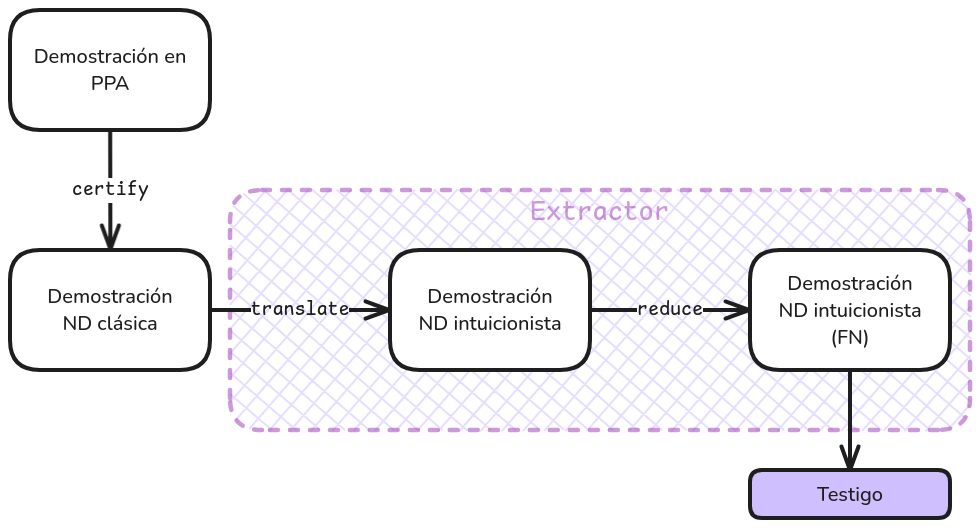
\includegraphics[scale=0.35]{img/fri-extract-strategy.png}
    \centering
    \caption{Estrategia de extracción de testigos}
    \label{fri:fig:strat}
\end{figure}

\section{Traducción de Friedman}

\subsection{Traducción de doble negación}

Existen muchos métodos que permiten embeber la lógica clásica en la
intuicionista \duda{citar?}. Un mecanismo general es la traducción de
\textbf{doble negación}, que tiene distintas variaciones. Una es la
\textit{Gödel-Gentzen} \cite{Avigad1998-FEFOFD}

\begin{definition}[Traducción \textit{Gödel-Gentzen}] Dada una fórmula $\form$
se asocia con otra $\gN{\form}$. La traducción se define por inducción
estructural.
    \begin{align*}
        \gN{\fFalse} &= \fFalse\\
        \gN{\fTrue} &= \fTrue\\
        \gN{\form} &= \fNot\fNot \form \quad \text{con $\form$ atómica}\\
        \gN{(\form \fAnd \formTwo)} &= \gN{\form} \fAnd \gN{\formTwo}\\
        \gN{(\form \fOr \formTwo)} &= \fNot(\fNot\gN{\form} \fAnd \fNot\gN{\formTwo})\\
        \gN{(\form \fImp \formTwo)} &= \gN{\form} \fImp \gN{\formTwo}\\
        \gN{(\forall \var . \form(\var))} &= \forall \var . \gN{\form(\var)}\\
        \gN{(\exists \var . \form(\var))} &= \fNot \forall \var . \fNot \gN{\form(\var)}
    \end{align*}
\end{definition}


\begin{definition}[Traducción de contextos]
    Se extiende a contextos de la forma esperable
    \[
        \gN{\ctx} = \{\gN{\form} \mid \form \in \ctx \}.
    \]
\end{definition}

\begin{notation*}
    Notamos,    
    \begin{itemize}
        \item $\judgC$ para expresar que un juicio es derivable en lógica clásica,
        y $\judgI$ para intuicionista.
        \item $\someProof \proves \ctx \judG \form$ para expresar que $\someProof$ es una demostración de $\ctx \judG \form$. Equivalente a
            \AxiomC{$\someProof$}
            \noLine
            \UnaryInfC{$\ctx \judG \form$}
            \DisplayProof
    \end{itemize}
\end{notation*}

\begin{theorem}
    Si tenemos $\ctx \judgC \form$, luego $\gN{\ctx} \judgI \gN{\form}$.
\end{theorem}

Dada una demostración en lógica clásica, podemos obtener una en lógica
intuicionista de su traducción. Pero esto no es exactamente lo que queremos,
pues si quisiéramos extraer un testigo de una demostración de la fórmula
$\exists \var. \pred(\var)$, al traducirla nos quedaría
\(
    \gN{(\exists \var. \pred(\var))}
        = \fNot \forall \var . \fNot\fNot\fNot \pred(\var),
\)
que si bien su demostración sería intuicionista (y por lo tanto constructiva),
como no es de un $\exists$ al normalizarla no podremos hacer la extracción.

\subsection{El truco de Friedman}

La idea de Friedman \cite{miquel-friedman} es generalizar la traducción
Gödel-Gentzen reemplazando la negación intuicionista $\fNot \form \equiv A
\rightarrow \bot$ por una relativa $\fNotR \form \equiv \form \rightarrow R$ que
está parametrizada por una fórmula arbitraria $R$. Esto nos va a permitir, con
una elección inteligente de $R$, traducir una demostración clásica de una
fórmula a una intuicionista, y usarla para demostrar \textbf{la fórmula
original}. Esto nos permite reducirla y hacer la extracción. No va a ser posible para cualquier fórmula, sino las de una clase particular (de la forma 
$\forall \varTwo_1 \dots \forall \varTwo_m . \exists \var_1 \dots \exists \var_k . \form$ o $\classPiTwo$)

\begin{definition}[Jerarquía aritmética de fórmulas]
    Clasifica las fórmulas en dos clases: $\classPi{n}$ y
    $\classSigma{n}$. Se define por inducción en $n$.

    \begin{itemize}
        \item Si $\anyForm$ es equivalente a una fórmula sin cuantificadores, está en
        $\classPi{0}$ y $\classSigma{0}$.
        \item Sean las clasificaciones $\classPi{n}$ y $\classSigma{n}$. Definimos para $n+1$.
        \begin{itemize}
            \item Si $\anyForm$ es equivalente a una formula de la forma $\exists
            \var_1 \dots \exists \var_k. \anyFormTwo$ donde $\anyFormTwo$ es
            $\classPi{n}$, entonces $\anyForm$ es asignada la clasificación $\classSigma{n+1}$.
    
            \item Si $\anyForm$ es equivalente a una formula de la forma $\forall
            \var_1 \dots \forall \var_k. \anyFormTwo$ donde $\anyFormTwo$ es
            $\classSigma{n}$, entonces $\anyForm$ es asignada la clasificación $\classPi{n+1}$.
        \end{itemize}
    \end{itemize}

    Una fórmula de $\classSigma{n}$ es equivalente a una que comienza con
    cuantificadores existenciales y alterna $n-1$ veces entre series de
    universales y existenciales. Mientras que una $\classPi{n}$ es análoga pero
    comenzando con universales.
    
    Las dos que más nos interesan son:
    \begin{itemize}
        \item $\classSigmaOne$: fórmulas de la pinta $\exists \var_1 \dots
        \exists \var_k . \anyForm$.
        \item $\classPiTwo$: fórmulas de la pinta $\forall \varTwo_1 \dots \forall \varTwo_m . \exists \var_1 \dots \exists \var_k . \anyForm$
    \end{itemize}

    

    Una intuición detrás de los nombres de las clases puede ser
    \begin{itemize}
        \item $\Sigma$ es una sumatoria, que se puede interpretar como
        disyunciones (en el sentido del álgebra de Boole), y generalizar con un existencial.
        \item $\Pi$ análogamente pero con productoria, conjunciones y universales.
    \end{itemize}
\end{definition}

\begin{definition}[Traducción de doble negación relativizada]
    \begin{align*}
        \transDNeg{\bot} &= \bot\\
        \transDNeg{\form} &= \fNotR\fNotR \form
            \quad \text{con $\form$ atómica}\\
        \transDNeg{(\fNot \form)} &= \fNot \transDNeg{\form}\\
        \transDNeg{(\form \fAnd \formTwo)} &= \transDNeg{\form} \fAnd \transDNeg{\formTwo}\\
        \transDNeg{(\form \fOr \formTwo)} &= \fNotR(\fNotR\transDNeg{\form} \fAnd \fNotR\transDNeg{\formTwo})\\
        \transDNeg{(\form \rightarrow \formTwo)} &= \transDNeg{\form} \rightarrow \transDNeg{\formTwo}\\
        \transDNeg{(\forall x . \form)} &= \forall x . \transDNeg{\form}\\
        \transDNeg{(\exists x . \form)} &= \fNotR \forall x . \fNotR \transDNeg{\form}
    \end{align*}
\end{definition}

\begin{theorem}
    \label{fri:thm:dneg-trans-classic-int}
    Si $\ctx \judgC \form$, luego $\transDNeg{\ctx} \judgI \transDNeg{\form}$
\end{theorem}
\begin{proof}
    Dada una demostración en deducción natural clásica $\ctx \judgC \form$, podemos traducirla recursivamente extendiendo la traducción de fórmulas a reglas de inferencia, así generando una demostración de $\transDNeg{\ctx} \judgI \transDNeg{\form}$.
    Este proceso está descrito en detalle en \fullref{fri:sec:proof-trans}
\end{proof}

Vamos a enunciar diferentes versiones de la traducción de Friedman en orden de sofisticación. No solo ayuda a entenderla, sino que también fue el mismo enfoque con el que las implementamos.

\begin{enumerate}
    \item \textbf{Fórmulas $\classSigmaOne$ atómicas} (\namedref{fri:thm:fri-sigmaone}):
    \[
        \exists \var . \form(\var) \text{ con } \form(\var) \text{ atómica.} 
    \]
    \item \textbf{Fórmulas $\classPiTwo$ atómicas} (\namedref{fri:thm:fri-pitwo}):
    
    \[
        \forall \varTwo_1 \dots \forall \varTwo_n . \exists \var . \form(\var, \varTwo_1, \dots, \varTwo_n) \text{ con } \form(\dots) \text{ atómica}.
    \]

    \item \textbf{Fórmulas $\classPiTwo$ no atómicas} (\namedref{fri:thm:fri-pitwo-general}):
    
    \[
    \forall \varTwo_1 \dots \forall \varTwo_n . \exists \var . \anyForm(\var, \varTwo_1, \dots, \varTwo_n) \text{ con } \anyForm(\dots) \text{ no atómica}.
    \]
    
    Por ejemplo, podría ser $\pred(x) \fAnd \predTwo(\varTwo_1, \dots, \varTwo_n)$.
    Pero no podrá ser cualquier fórmula, por ej. no $\fNot(\pred(x) \fAnd \predTwo(\varTwo_1, \dots, \varTwo_n))$. En \todo{Cita} damos una caracterización.
\end{enumerate}

\begin{theorem}[Traducción de Friedman para fórmulas $\classSigmaOne$]
    \label{fri:thm:fri-sigmaone}

    Sea $\someProof$ una demostración clásica de $\exists \var . \form$, y
    $\form$ una fórmula atómica.
    Si tenemos
    \[
        \ctx \judgC \exists \var . \form,
    \]
    luego, podemos generar una demostración intuicionista de \textit{la misma fórmula}
    \[
        \transDNeg{\ctx} \judgI \exists \var . \form.
    \]
\end{theorem}
\begin{proof}

Aplicando la traducción, tenemos que

\begin{gather*}
    \transDNeg{\big(
        \someProof \proves \ctx \judgC \exists \var . \form
    \big)}\\
    \verteq\\
    \transDNeg{\someProof} \proves \transDNeg{\ctx} \judgI \fNotR \forall \var . \fNotR \fNotR \fNotR \form
\end{gather*}

luego, tomando $R = \exists \var . \form$ la fórmula que buscamos probar,

\begin{align*}
    \transDNeg{\someProof} \proves & \transDNeg{\ctx} \judgI \fNotR \forall \var . \fNotR \fNotR \fNotR \form\\
    \iff & \transDNeg{\ctx} \judgI \fNotR \forall \var . \fNotR \form
        &&(\text{\namedref{fri:lemma:tnegr-elim}})\\
    =\ &\transDNeg{\ctx} \judgI (\forall \var . (\form \rightarrow R)) \rightarrow R
        &&(\fNotR \form = \form \fImp R)\\
    =\ &\transDNeg{\ctx} \judgI (\forall \var . (\form \rightarrow \exists \var . \form)) \rightarrow \exists \var . \form && (R = \exists \var \form)\\
    \Rightarrow\ &\transDNeg{\ctx} \judgI \exists \var . \form
        && (\text{\namedref{fri:obs:forall-exists}})
\end{align*}

En deducción natural,

\begin{prooftree}
    \def\defaultHypSeparation{\hskip .1in}
    \AxiomC{$\transDNeg{\someProof}$}
    \noLine
    \UnaryInfC{\(
        \transDNeg{\ctx} \judgI \fNotR \forall \var \fNotR \transDNeg{\form}
    \)}
    \AxiomC{}
    \RL{\ruleTNegRI}
    \admissibleRuleLine
    \UnaryInfC{$\transDNeg{\ctx}, \fNotR \form \judgI \fNotR \fNotR \fNotR \form$}
    \AxiomC{}
    \RL{\ruleAx}
    \UnaryInfC{$\transDNeg{\ctx}, \form \judgI \form$}
    \RL{\ruleExistsI}
    \UnaryInfC{$\transDNeg{\ctx}, \form \judgI R = \exists \var \form$}
    \RL{\ruleImpI}
    \UnaryInfC{$\transDNeg{\ctx} \judgI \fNotR \form$}
    \RL{\ruleCut}
    \admissibleRuleLine
    \BinaryInfC{$\transDNeg{\ctx} \judgI \fNotR \fNotR \fNotR \form$}
    \RL{\ruleForallI}
    \UnaryInfC{\(
        \transDNeg{\ctx} \judgI \forall \var \fNotR \transDNeg{\form}
    \)}
    \RL{\ruleImpE}
    \BinaryInfC{$\transDNeg{\ctx} \judgI \exists \var . \form$}
\end{prooftree}
\end{proof}

\begin{obs}
    En la demostración del \namedref{fri:thm:fri-sigmaone} y las de esta sección, luego de la traducción de Friedman, todas las demostraciones deben ser intuicionistas para que sigan siendo constructivas.
\end{obs}

\begin{lemma}[Eliminación de triple negación relativa]\label{fri:lemma:tnegr-elim}
    $\fNotR\fNotR\fNotR \form \iff \fNotR \form$ y lo demostramos como dos reglas admisibles, una para cada lado

    \begin{multicols}{2}
        \begin{prooftree}
            \AxiomC{}
            \RL{\ruleTNegRE}
            \admissibleRuleLine
            \UnaryInfC{$\fNotR\fNotR\fNotR \form \judgI \fNotR \form$}
        \end{prooftree}
    
        \begin{prooftree}
            \AxiomC{}
            \RL{\ruleTNegRI}
            \admissibleRuleLine
            \UnaryInfC{$\fNotR \form \judgI \fNotR\fNotR\fNotR \form$}
        \end{prooftree}
    \end{multicols}
\end{lemma}
\begin{proof}

    Primero \ruleTNegRI{}

    \begin{prooftree}
        \AxiomC{}
        \RL{\ruleAx}
        \UnaryInfC{$\fNotR \form, \fNotR\fNotR \form \judgI \fNotR \fNotR \form$}
        \AxiomC{}
        \RL{\ruleAx}
        \UnaryInfC{$\fNotR \form, \fNotR\fNotR \form \judgI \fNotR \form$}
        \RL{\ruleImpE}
        \BinaryInfC{$\fNotR \form, \fNotR\fNotR \form \judgI R$}
        \RL{\ruleImpI}
        \UnaryInfC{$\fNotR \form \judgI \fNotR\fNotR\fNotR \form$}
    \end{prooftree}

    Ahora \ruleTNegRE{}

    \begin{prooftree}
        \AxiomC{}
        \RL{\ruleAx}
        \UnaryInfC{$\fNotR\fNotR\fNotR \form, \form \judgI \fNotR\fNotR\fNotR \form$}
        \AxiomC{}
        \RL{\ruleAx}
        \UnaryInfC{$\ctx \judgI \fNotR \form$}
        \AxiomC{}
        \RL{\ruleAx}
        \UnaryInfC{$\ctx \judgI \form$}
        \RL{\ruleImpE}
        \BinaryInfC{$\ctx = \fNotR\fNotR\fNotR \form, \form, \fNotR \form \judgI R$}
        \RL{\ruleImpI}
        \UnaryInfC{$\fNotR\fNotR\fNotR \form, \form \judgI \fNotR\fNotR \form$}
        \RL{\ruleImpE}
        \BinaryInfC{$\fNotR\fNotR\fNotR \form, \form \judgI R$}
        \RL{\ruleImpI}
        \UnaryInfC{$\fNotR\fNotR\fNotR \form \judgI \fNotR \form$}
    \end{prooftree}
\end{proof}

\begin{obs}\label{fri:obs:forall-exists}
    $\judgI \forall \var (\form \rightarrow \exists \var \form)$.
    Trivialmente, para cualquier $\var$ si vale $\form$ entonces va a existir un $\var$ tal que valga $\form$.
\end{obs}

\todo{IDem pero en ND, y también para $\forall$}


\begin{theorem}[Traducción de Friedman para fórmulas $\classPiTwo$ atómicas]
    \label{fri:thm:fri-pitwo}

    Sea $\someProof$ una demostración clásica de
    \(
        \forall \varTwo_1 \dots \forall \varTwo_n .
        \exists \var .
        \form(\var, \varTwo_1, \dots, \varTwo_n)
    \)
    y $\form(\dots)$ una fórmula atómica

    Si tenemos
    \[
        \ctx \judgC
        \forall \varTwo_1 \dots \forall \varTwo_n .
        \exists \var .
        \form(\var, \varTwo_1, \dots, \varTwo_n),
    \]
    podemos generar una demostración intuicionista de la misma fórmula
    \[
        \transDNeg{\ctx} \judgI
        \forall \varTwo_1 \dots \forall \varTwo_n .
        \exists \var .
        \form(\var, \varTwo_1, \dots, \varTwo_n).
    \]
\end{theorem}
\begin{proof}
    \todo{proof}
\end{proof}

\subsubsection{Formulas no atómicas}
Es igual al anterior, pero para una fórmula arbitraria. Queremos generalizar r intro. Lema

\begin{lemma}[Introducción de $\fNotR$]
    No vale siempre.
\end{lemma}

\begin{theorem}[Traducción de Friedman para fórmulas $\classSigmaOne$ en general]
    \label{fri:thm:fri-pitwo-general}

    Sea $\someProof$ una demostración clásica de\(
        \forall \varTwo_1 \dots \forall \varTwo_n .
        \exists \var .
        \anyForm(\var, \varTwo_1, \dots, \varTwo_n)
    \), y
    $\anyForm(\var, \varTwo_1, \dots, \varTwo_n)$ una fórmula no atómica.
    Si tenemos
    \[
        \ctx \judgC 
        \forall \varTwo_1 \dots \forall \varTwo_n .
        \exists \var .
        \anyForm(\var, \varTwo_1, \dots, \varTwo_n),
    \]
    podemos generar una demostración intuicionista de la misma fórmula
    \[
        \transDNeg{\ctx} \judgI
        \forall \varTwo_1 \dots \forall \varTwo_n .
        \exists \var .
        \anyForm(\var, \varTwo_1, \dots, \varTwo_n).
    \]
\end{theorem}
\begin{proof}
    \todo{}
\end{proof}

\subsection{Traducción de demostraciones}
\label{fri:sec:proof-trans}

En \fullref{fri:thm:dneg-trans-classic-int} se introduce la necesidad de extender la traducción de doble negación relativizada de fórmulas a demostraciones, para poder convertir una demostración clásica a intuicionista. En esta sección lo vemos más en detalle.

La conversión se efectúa por inducción estructural en la demostración. Para cada regla de inferencia que demuestra $\form$, se genera una demostración a partir de ella para demostrar $\transDNeg{\form}$. La estrategia para hacerlo es similar para todas: usar la hipótesis inductiva para convertir las sub-demostraciones, y usarlas para generar la nueva demostración. Pero hay algunas que requieren un truco. Solo mostramos las interesantes.

\begin{itemize}
    \item \ruleAndI{} (\namedref{fri:lemma:trad-and-i}), \ruleAndEOne{}, \ruleAndETwo{}, \ruleImpI{}, \ruleImpE{}, 
    \ruleOrIOne{}, \ruleOrITwo{}, \ruleForallI{}, \ruleForallE{}, \ruleNotI{}, \ruleNotE{}, \ruleTrueI{}, \ruleAx{} son todas similares entre sí, por lo que solo mostramos una.
    \item \ruleExistsI{} (\namedref{fri:lemma:trad-exists-i}) es una regla simple pero más interesante que las anteriores, por la traducción de $\exists$.
    \item \ruleLEM{} (\namedref{fri:lemma:trad-lem}) es sumamente interesante, ya que se encuentra en el corazón de la traducción al ser la parte clave: ¿cómo traducimos el principio de razonamiento clásico que lo separa de la lógica intuicionista?
    \item \ruleFalseE{} (\namedref{fri:lemma:trad-false-e})  se prueba como lema por inducción estructural en la fórmula a demostrar.
    \item \ruleOrE{} (\namedref{fri:lemma:trad-or-e}) y \ruleExistsE{} son análogos y requieren un truco: usar la eliminación de la doble negación. Si bien al ser un principio de razonamiento clásico no vale para lógica intuicionista (por ser equivalente a LEM), lo que si vale es la eliminación de la doble negación relativizada: \ruleDnegRE{} (\namedref{fri:lemma:dnegr-e}).
\end{itemize}

\begin{lemma}[Traducción de \ruleAndI{}]
    \label{fri:lemma:trad-and-i}
    Dada una aparición de la regla \ruleAndI{},

    \begin{prooftree}
        \AxiomC{$\someProof_\form$}
        \noLine
        \UnaryInfC{$\ctx \judgI \form$}
        \AxiomC{$\someProof_\formTwo$}
        \noLine
        \UnaryInfC{$\ctx \judgI \formTwo$}
        \RL{\ruleAndI}
        \BinaryInfC{$\ctx \judgI \form \wedge \formTwo$}
    \end{prooftree}

    es posible traducirla generando una demostración de $\tdn{(\form \fAnd \formTwo)} = \tdn{\form} \fAnd \tdn{\formTwo}$.
\end{lemma}
\begin{proof}
    Por hipótesis inductiva, tenemos que
    \begin{itemize}
        \item \(
            \tdn{\someProof_\form} \proves
            \tdn{\ctx} \judgI
            \tdn{\form}
        \) y
        \item \(
            \tdn{\someProof_\formTwo} \proves
            \tdn{\ctx} \judgI
            \tdn{\formTwo}
        \)
    \end{itemize}

    Luego, podemos generar una demostración de $\tdn{\form} \fAnd \tdn{\formTwo}$

    \begin{prooftree}
        \AxiomC{$\tdn{\someProof_\form}$}
        \noLine
        \UnaryInfC{$\tdn{\ctx} \judgI \tdn{\form}$}
        \AxiomC{$\tdn{\someProof_\formTwo}$}
        \noLine
        \UnaryInfC{$\tdn{\ctx} \judgI \tdn{\formTwo}$}
        \RL{\ruleAndI}
        \BinaryInfC{$\tdn{\ctx} \judgI \tdn{\form} \fAnd \tdn{\formTwo}$}
    \end{prooftree}
\end{proof}

\begin{lemma}[Traducción de \ruleExistsI{}]
    \label{fri:lemma:trad-exists-i}
    \todo{Enunciar y demostrar}
\end{lemma}

\begin{lemma}[Traducción de \ruleLEM{}]
    \label{fri:lemma:trad-lem}
    \todo{Enunciar y demostrar}
\end{lemma}

\begin{lemma}[Traducción de \ruleFalseE{}]
    \label{fri:lemma:trad-false-e}
    \todo{Enunciar y demostrar}
\end{lemma}

\begin{lemma}[Eliminación de doble negación relativizada (\ruleDnegRE{})]
    \label{fri:lemma:dnegr-e}
    \todo{Enunciar y demostrar}
\end{lemma}

\begin{lemma}[Traducción de \ruleOrE{}]
    \label{fri:lemma:trad-or-e}
    \todo{Enunciar y demostrar}
\end{lemma}

\subsection{Manteniendo el contexto}

Problema con normalización: axiomas, hay que traducirlos para que la traducción de Friedman funcione. Solución? Dejar los axiomas originales y demostrar su traducción. No funciona siempre.

\begin{lemma}[Introducción de la traducción $\fNot\fNot$]
    Se reduce a transintro
\end{lemma}

\todo{Enunciar y demostrar}

\section{Normalización}

existe curry howard \cite{curry-howard-isomorphism}, relación entre deducción
natural y cálculo lambda. Luego, la normalización de demostraciones es el
isomorfismo de la semántica del cálculo lambda.

evitar \textit{detours}, leer más en el libro de curry howard

Mostrar ejemplo del and de curry howard.

\subsection{Sustituciones}

substHyp y substVar, la especificación matemática (y descripción de los problemas)

\subsection{Reglas de reducción}

Mostrar un par que sean intersantes, no todas.

\subsection{Estrategia de reducción}

...

\subsection{Limitaciones}

No funciona para todas las demostraciones, porque hay algunas reducciones que no implementamos.

\section{Otros métodos de extracción}

\todo{Hablar sobre y citar classical realizability, no tengo ni idea.}

Buena intro acá https://www.degruyter.com/document/doi/10.1515/9783110324921.11/html?lang=en

In the past years, many computational interpretations of Classical Arithmetic havebeen put forward.  Under a first classification, they fall into two large categories:directandindirectinterpretations.   Among  the  indirect  interpretations  one  findsthe  negative  translations  followed  either  by  Dialectica  interpretations  [13],  [30](see e.g.   Kohlenbach [19]) or by intuitionistic realizability interpretations com-bined with Friedman’s translation [13] (see e.g. Berger and Schwichtenberg [10]).Among the direct interpretations, there are different versions of Classical Realiz-ability (Krivine’s [22] and Avigad’s [6]), there is Coquand game semantics [11],

\chapter{La herramienta \texttt{ppa}}
\label{chap:ppa-tool}

\begin{figure}[H]
\begin{multicols}{2}
\begin{minted}{haskell}
type VarId = String
type FunId = String
type PredId = String
type HypId = String

data Term
    = TVar VarId
    | TMetavar Metavar
    | TFun FunId [Term]

data Form
    = FPred PredId [Term]
    | FAnd Form Form
    | FOr Form Form
    | FImp Form Form
    | FNot Form
    | FTrue
    | FFalse
    | FForall VarId Form
    | FExists VarId Form
\end{minted}
\end{multicols}
\caption{Modelado de fórmulas y términos de LPO}
\end{figure}


Las meta-variables se usan para unificación, que es parte del solver de PPA. Ver
más en \fullref{ppa:sec:unification}

\begin{figure}[H]
    
\begin{multicols}{2}
\begin{minted}{haskell}
data Proof =
    | PAx HypId
    | PAndI
        { proofLeft :: Proof
        , proofRight :: Proof
        }
    | PAndE1
        { right :: Form
        , proofAnd :: Proof
        }
    | PAndE2
        { left :: Form
        , proofAnd :: Proof
        }
    | POrI1
        { proofLeft :: Proof
        }
    | POrI2
        { proofRight :: Proof
        }
    | POrE
        { left :: Form
        , right :: Form
        , proofOr :: Proof
        , hypLeft :: HypId
        , proofAssumingLeft :: Proof
        , hypRight :: HypId
        , proofAssumingRight :: Proof
        }
    | PImpI
        { hypAntecedent :: HypId
        , proofConsequent :: Proof
        }
    | PImpE
        { antecedent :: Form
        , proofImp :: Proof
        , proofAntecedent :: Proof
        }
    | PNotI
        { hyp :: HypId
        , proofBot :: Proof
        }
    | PNotE
        { form :: Form
        , proofNotForm :: Proof
        , proofForm :: Proof
        }
    | PTrueI
    | PFalseE
        { proofBot :: Proof
        }
    | PLEM
    | PForallI
        { newVar :: VarId
        , proofForm :: Proof
        }
    | PForallE
        { var :: VarId
        , form :: Form
        , proofForall :: Proof
        , termReplace :: Term
        }
    | PExistsI
        { inst :: Term
        , proofFormWithInst :: Proof
        }
    | PExistsE
        { var :: VarId
        , form :: Form
        , proofExists :: Proof
        , hyp :: HypId
        , proofAssuming :: Proof
        }
\end{minted}        
\end{multicols}
\caption{Modelado de reglas de inferencia para demostraciones}
\end{figure}


El modelado de las reglas de inferencia omite varios detalles que están
implícitos y serán inferidos por el algoritmo de chequeo. De esa forma las
demostraciones son más fáciles de escribir y generar. Por ejemplo,
\texttt{PImpI} no especifica en su modelo cuál es la implicación que se está
introduciendo, dado que durante el chequeo debería ser la fórmula actual a
demostrar

\section{Compiladores}
\begin{itemize}
    \item Primer de compiladores en general y sus frontends
    \item Parser generators en general. LR/LALR
    \item Happy. Alex.
    \item Sintaxis BNF en apéndice (el archivo). Incluir el archivo Alex/happy? Es cortito
\end{itemize}

\chapter{Conclusiones}

En este trabajo presentamos el lenguaje \ppaLang{} junto con los detalles de su
implementación en \ppaTool{}. Primero dimos una definición completa del sistema
lógico de deducción natural, junto con ejemplos de demostraciones de una
teoría de estudiantes. Se presentan también algunos ajustes que tuvimos que
hacer al sistema para implementarlo: etiquetado de hipótesis (y cómo afecta eso
a las reglas de inferencia) y relajamiento de restricciones sobre variables
libres en el contexto. Describimos cómo implementamos los algoritmos de chequeo,
alfa equivalencia de forma lineal y sustitución sin capturas de forma lineal.

Dimos un manual de usuario para el lenguaje \ppaLang{}, explicando como
escribir demostraciones y cómo usar el mecanismo de demostración principal
\lstinline{by}. Damos una demostración completa que extiende el ejemplo de
estudiantes y muestra diferentes capacidades del lenguaje. También se listan
todos los comandos, ejemplos funcionales para cada uno, y su relación con las
reglas de inferencia de deducción natural. Profundizamos en la implementación
del certificador y cómo están implementadas cada una de las partes de la
interfaz. Centralmente el \textit{solver} usado por debajo del \lstinline{by}.

Finalmente vimos una implementación posible de eliminación de testigos
existenciales. Mencionamos las limitaciones al tratar de hacerlo de forma
directa sobre lógica clásica, las distintas versiones de la traducción de
Friedman según el tipo de fórmula a demostrar, y las limitaciones que se
presentaron (no se podrá asumir cualquier axioma, ni demostrar cualquier fórmula
$\classPiTwo$). Luego describimos cómo a partir del isomorfismo Curry-Howard
pudimos implementar un mecanismo de normalización de demostraciones, que también
presentó limitaciones (no todas las demostraciones podrán ser llevadas a su
forma normal) y requirió cambios en la estrategia de reducción de una sencilla a
una más sofisticada (Gross-Knuth) debido al tamaño de las demostraciones.

El principal aporte del trabajo es la implementación práctica de un método de
extracción directo mediante el uso de la traducción de Friedman y la
normalización usual de la lógica intuicionista.

\section{Trabajo futuro}

Surgieron varias líneas de trabajo futuro, que quedaron fuera del alcance de la
tesis. Las listamos a continuación.

% TODO: Tipos?

\begin{itemize}
    \item \textbf{Modelar de forma nativa inducción e igualdad}: las teorías que se pueden axiomatizar están limitadas al no poder
    representar inducción de forma nativa (como predica sobre predicados, es
    lógica de segundo orden). Si se puede axiomatizar de forma adhoc, como
    predicados escritos a mano en cada programa, pero sería más amigable de
    estar como regla de inferencia y a lo largo de todo el programa. También se
    podría agregar de forma nativa la noción de \textit{igualdad}.
    \item \textbf{Sofisticar \textit{solver} del by}: en
    \fullref{ppa-cert:sec:expressiveness} se mencionan las limitaciones del
    \textit{solver} usado por el \lstinline{by}. Una funcionalidad que quedó
    afuera pero sería sencilla de agregar es que no solo se busque eliminar los
    $\forall$ consecutivos de \textit{una} hipótesis, sino que el proceso sea
    recursivo: que exhaustivamente intente de eliminar los $\forall$ de todas
    las combinaciones de hipótesis posibles.
    \item \textbf{Mejorar a PPA como lenguaje de programación}: el
    lenguaje PPA no brinda soporte para tener un ecosistema. Se pueden agregar
    muchas funcionalidades que mejorarían la calidad de vida del desarrollador
    como permitir importar archivos o módulos e implementar una biblioteca
    estándar de teorías y teoremas.
    \item \textbf{Refinar demostración usada para traducción}: en la traducción de Friedman introducimos dos lemas centrales:
    $\formTwo \judgI \tdn{\formTwo}$ \fullref{fri:lemma:trans-intro}, y
    $\fNotR \form \judgI \fNotR \tdn{\form}$
    \fullref{fri:lemma:notr-trans-intro}. El primero se reduce al segundo.
    El segundo no vale siempre, pero demostramos un subconjunto de todas las
    demostraciones válidas. Podríamos refinarlo aún más, lo que permitiría usar
    más clases de axiomas para las demostraciones que se quiera extraer
    testigos.
    \item \textbf{Implementar versión completa de reducción de demostraciones}:
    en \fullref{fri:norm:sec:limitations} vimos una demostración para la que no
    se puede llegar a una forma normal, evitando la extracción de testigos en un
    caso en el que debería ser posible. Se podría extender la implementación de
    la reducción para incluir más tipos de reglas, así haciendo que sea completa.
    \item \textbf{Mejorar reporte de errores}: los errores reportados por la
    herramienta en general son muy rústicos, implementativos y de bajo nivel. Se
    podrían hacer más amigables y accionables, ayudando a resolver problemas sin
    saber cómo funciona internamente la herramienta.
\end{itemize}

%%%% BIBLIOGRAFIA
\backmatter
\printbibliography

\end{document}